% This must be in the first 5 lines to tell arXiv to use pdfLaTeX, which is strongly recommended.
\pdfoutput=1
% In particular, the hyperref package requires pdfLaTeX in order to break URLs across lines.

\documentclass[11pt]{article}

% Change "review" to "final" to generate the final (sometimes called camera-ready) version.
% Change to "preprint" to generate a non-anonymous version with page numbers.
\usepackage[final]{acl}

% Standard package includes
\usepackage{times}
\usepackage{latexsym}

% For proper rendering and hyphenation of words containing Latin characters (including in bib files)
\usepackage[T1]{fontenc}
% For Vietnamese characters
% \usepackage[T5]{fontenc}
% See https://www.latex-project.org/help/documentation/encguide.pdf for other character sets

% This assumes your files are encoded as UTF8
\usepackage[utf8]{inputenc}

% This is not strictly necessary, and may be commented out,
% but it will improve the layout of the manuscript,
% and will typically save some space.
\usepackage{microtype}

% This is also not strictly necessary, and may be commented out.
% However, it will improve the aesthetics of text in
% the typewriter font.
\usepackage{inconsolata}

%Including images in your LaTeX document requires adding
%additional package(s)
\usepackage{graphicx}

% Allows for side by side images
\usepackage{subcaption}


% Defined tick and cross emojis
\usepackage{pifont}

\newcommand{\cmark}{\ding{51}}  % Define command for tick mark
\newcommand{\xmark}{\ding{55}}  % Define command for cross mark

% To move caption of tables to the top
\usepackage{float}
%\floatstyle{plaintop}
%\restylefloat{table}

% To allow for left aligned columns
\usepackage{array}

% To allow multirow in tables
\usepackage{multirow}

% To allow for math symbols
\usepackage{amsmath}
\usepackage{amsfonts}

% For prompt listings
\usepackage{listings}
\lstset{
  backgroundcolor=\color{gray!8},
  basicstyle=\ttfamily,
  columns=fullflexible
}

% For algorithms 
\usepackage[ruled,vlined]{algorithm2e}


% \usepackage{hyperref}
\usepackage{url}
\usepackage{xspace}
\usepackage{caption}
\usepackage{wrapfig}
%\usepackage{algorithm}
\usepackage{algpseudocode}
\usepackage{amsmath,amssymb}
\usepackage{float}
\usepackage{graphicx}
\usepackage{csquotes}
\usepackage{xcolor}
\usepackage{multirow}
\usepackage{multicol}
\usepackage{wrapfig,lipsum,booktabs}
\usepackage{makecell}
\usepackage{wrapfig}
\usepackage{array}
\usepackage{color, colortbl}
\usepackage{pifont}
\usepackage{enumitem}
% \usepackage[font=small,labelfont=bf]{caption}
\usepackage{inconsolata}
\usepackage{subcaption}
% \usepackage[hidelinks,colorlinks=true,linkcolor=blue,citecolor=blue]{hyperref}
\usepackage{xcolor}
% \usepackage{ulem}
\usepackage[normalem]{ulem} % normalem avoids changing \emph{} to underlined
\usepackage{soul}
% \usepackage{soulutf8}
% \usepackage{luacolor}
% \usepackage[soul]{lua-ul}
\newcommand{\ctext}[3][RGB]{%
  \begingroup
  \definecolor{hlcolor}{#1}{#2}\sethlcolor{hlcolor}%
  \hl{#3}%
  \endgroup
}

\usepackage{bm}


% If the title and author information does not fit in the area allocated, uncomment the following
%
%\setlength\titlebox{<dim>}
%
% and set <dim> to something 5cm or larger.

\title{Dynamic Rewarding with Prompt Optimization Enables \\ Tuning-free Self-Alignment of Language Models}


% Author information can be set in various styles:
% For several authors from the same institution:
% \author{Author 1 \and ... \and Author n \\
%         Address line \\ ... \\ Address line}
% if the names do not fit well on one line use
%         Author 1 \\ {\bf Author 2} \\ ... \\ {\bf Author n} \\
% For authors from different institutions:
% \author{Author 1 \\ Address line \\  ... \\ Address line
%         \And  ... \And
%         Author n \\ Address line \\ ... \\ Address line}
% To start a separate ``row'' of authors use \AND, as in
% \author{Author 1 \\ Address line \\  ... \\ Address line
%         \AND
%         Author 2 \\ Address line \\ ... \\ Address line \And
%         Author 3 \\ Address line \\ ... \\ Address line}

% \author{First Author \\
%   Affiliation / Address line 1 \\
%   Affiliation / Address line 2 \\
%   Affiliation / Address line 3 \\
%   \texttt{email@domain} \\\And
%   Second Author \\
%   Affiliation / Address line 1 \\
%   Affiliation / Address line 2 \\
%   Affiliation / Address line 3 \\
%   \texttt{email@domain} \\
%   }


\author{%
Somanshu Singla\textsuperscript{$*\clubsuit$} \ 
Zhen Wang\thanks{Equal contribution}\textsuperscript{$\clubsuit$ $\spadesuit$} \
Tianyang Liu\textsuperscript{$\clubsuit$}\  
 \\ 
\textbf{ Abdullah Ashfaq\textsuperscript{$\clubsuit$} \
Zhiting Hu\textsuperscript{$\clubsuit$} \ 
Eric P. Xing\textsuperscript{$\spadesuit$ $\diamondsuit$}}  
\vspace{5pt} \\
\textsuperscript{$\clubsuit$}UC San Diego \
\textsuperscript{$\spadesuit$}MBZUAI \ \textsuperscript{$\diamondsuit$} CMU \\
\texttt{\{ssingla, zhw085\}@ucsd.edu}  
}


%\author{
%  \textbf{First Author\textsuperscript{1}},
%  \textbf{Second Author\textsuperscript{1,2}},
%  \textbf{Third T. Author\textsuperscript{1}},
%  \textbf{Fourth Author\textsuperscript{1}},
%\\
%  \textbf{Fifth Author\textsuperscript{1,2}},
%  \textbf{Sixth Author\textsuperscript{1}},
%  \textbf{Seventh Author\textsuperscript{1}},
%  \textbf{Eighth Author \textsuperscript{1,2,3,4}},
%\\
%  \textbf{Ninth Author\textsuperscript{1}},
%  \textbf{Tenth Author\textsuperscript{1}},
%  \textbf{Eleventh E. Author\textsuperscript{1,2,3,4,5}},
%  \textbf{Twelfth Author\textsuperscript{1}},
%\\
%  \textbf{Thirteenth Author\textsuperscript{3}},
%  \textbf{Fourteenth F. Author\textsuperscript{2,4}},
%  \textbf{Fifteenth Author\textsuperscript{1}},
%  \textbf{Sixteenth Author\textsuperscript{1}},
%\\
%  \textbf{Seventeenth S. Author\textsuperscript{4,5}},
%  \textbf{Eighteenth Author\textsuperscript{3,4}},
%  \textbf{Nineteenth N. Author\textsuperscript{2,5}},
%  \textbf{Twentieth Author\textsuperscript{1}}
%\\
%\\
%  \textsuperscript{1}Affiliation 1,
%  \textsuperscript{2}Affiliation 2,
%  \textsuperscript{3}Affiliation 3,
%  \textsuperscript{4}Affiliation 4,
%  \textsuperscript{5}Affiliation 5
%\\
%  \small{
%    \textbf{Correspondence:} \href{mailto:email@domain}{email@domain}
%  }
%}

\def\ours{\text{DRPO}\xspace}

\definecolor{forest green}{RGB}{34, 139, 34}

\renewcommand{\cmark}{\textcolor{forest green}{\ding{51}}}
\renewcommand{\xmark}{\textcolor{red}{\ding{55}}}

\newcommand{\zhen}[1]{\textcolor{red}{ZW: #1}}
\newcommand{\somanshu}[1]{\textcolor{green}{SS: #1}}
\newcommand{\tianyang}[1]{\textcolor{blue}{TL: #1}}


\begin{document}
\maketitle
局部感受野——对输入的某些连续时空特征具有选择性的神经元——存在于哺乳动物大脑的早期感觉区域。优化显式稀疏性或独立性标准的无监督学习算法复制了这些局部感受野的特征,但未能直接解释在没有高效编码的情况下,如何通过学习实现局部化,正如在深度神经网络的早期层中发生的那样,也可能在生物系统的早期感觉区域中发生。我们考虑了一种替代模型,在该模型中,局部感受野在没有显式自上而下效率约束的情况下出现——一个基于自然图像结构启发的数据模型训练的前馈神经网络。先前的研究确定了非高斯统计对局部化的重要性,但对于推动动态涌现的机制仍然存在未解之谜。我们通过推导单个非线性神经元的有效学习动力学来解决这些问题,精确说明输入数据的高阶统计特性如何驱动涌现的局部化,并证明这些有效动力学的预测可以扩展到多神经元设置。我们的分析为局部化的普遍性提供了一种替代解释,认为局部化是神经电路中学习的非线性动力学的结果。\smash{\footnotemark}\footnotetext{
实验和图形的复现代码请见
\url{https://github.com/leonlufkin/localization}.
}




\section{引言}

将大型语言模型(LLMs,~\citealt{brown2020language,chowdhery2023palm, touvron2023llama,achiam2023gpt})与人类伦理标准和实践预期对齐,对于防止意外后果并确保人工智能对社会的积极贡献至关重要。传统的对齐方法,如监督微调(SFT)和基于人类反馈的强化学习(RLHF)~\cite{bai2022constitutional, ouyang2022training},资源消耗大,并且需要大量的人类监督,限制了它们的可扩展性和实用性。随着LLM变得更加复杂和广泛应用,对成本效益高、标注效率高、快速适应的对齐策略的需求变得越来越迫切。

\begin{figure}
    \centering
    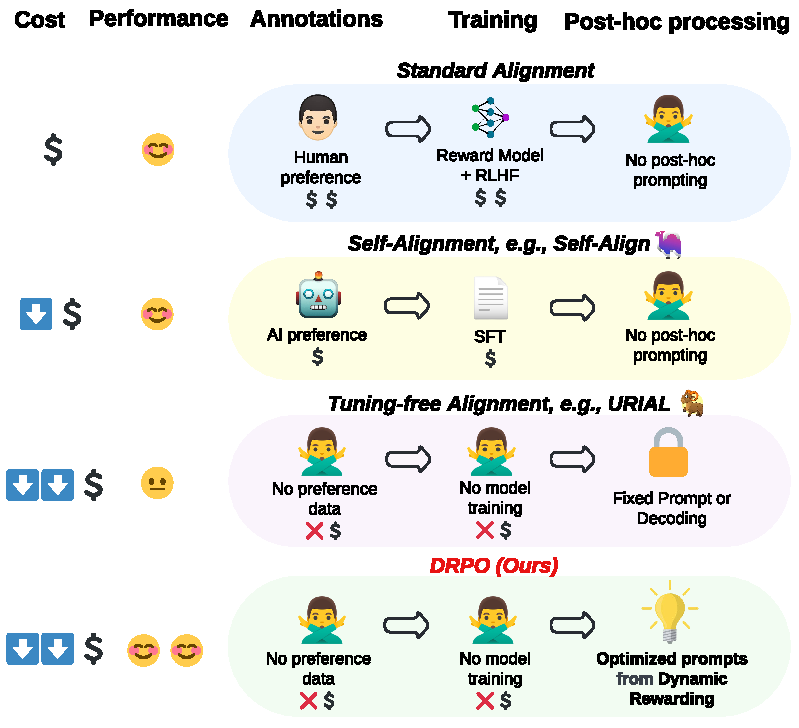
\includegraphics[width=1\linewidth]{images/DRPO_comparison.pdf}
    \vspace{-18pt}
    \caption{与其他LLM对齐范式的对比。 \ours结合了自我对齐和无需调优对齐的优点,能够实现自我改进和高效的成本效益,无需人工监督或额外的模型训练。}
    \vspace{-22pt}
    \label{fig:paradigm_comparison}
\end{figure}

自我对齐旨在通过利用模型本身来改善LLM对齐;例如,通过用模型生成的反馈代替人工反馈~\cite{lee2023rlaif},合成偏好数据~\cite{kim2023aligning, sun2024principle},或自我批评~\cite{bai2022constitutional}。尽管有这些进展,这些方法仍然需要大量资源,包括成本高昂且不稳定的RLHF调优,以及某些程度的人工监督,例如精心策划的对齐规则或上下文学习(ICL)提示~\cite{sun2024principle}。另一方面,如图~\ref{fig:paradigm_comparison}所示,最近的研究重点是无需调优的对齐,优先考虑极高的效率,而不需要承担任何调优成本。这些方法包括基于解码的对齐技术~\cite{li2023rain, wang2024inferaligner}或ICL对齐~\cite{han2023context, Lin2024ReAlign, zhao2024context}。然而,这些无需调优的方法通常是静态的(例如,依赖于固定的提示或奖励函数),因此缺乏适应性和自我改进能力,以实现更好的对齐。

为了结合这两种范式的优点,本文提出了\ours,动态奖励与提示优化(Dynamic Rewarding with Prompt Optimization),一种新的无需调优的LLM自我对齐方法。 \ours从近期对齐研究中的两个关键见解中汲取灵感。首先,表面对齐假设~\cite{zhou2024lima}表明,通过轻量级的调优或简单的提示,LLM可以有效地进行对齐~\cite{Lin2024ReAlign, zhao2024context}。其次,RLHF中的奖励模型往往对分布外样本的泛化能力较差~\cite{burns2023weak},而LLM因其出色的泛化能力,可以提供更有效的奖励和反馈来进行对齐。基于这些见解,\ours构建在基于搜索的提示优化(PO)框架之上~\cite{pryzant2023automatic, hao2023reasoning, wang2023promptagent},该框架使得LLM能够自我修正并自动生成详细的对齐指令,从而更加有效地引导模型行为,而无需依赖于任何人工偏好或模型训练。

\ours的核心创新在于其\textit{动态奖励}机制,与优化框架集成在一起。该机制允许基于LLM的奖励根据具体查询动态调整,有助于识别和解决模型的对齐盲点。例如,如果一个LLM因知识过时而假装回答一个需要最新新闻的问题,它的“知识限制”奖励将很低,并且对齐提示将相应地更新。我们将这种新方法应用于自动生成系统提示和ICL示例中的响应,证明其在提升对齐方面极为有效。

我们对8个近期的LLM进行了全面的实验,使用了标准的对齐基准\texttt{just-eval-instruct},该基准由多个对齐数据集中的问题组成。我们的结果表明,\ours能够有效地对齐基本模型和SFT/RLHF调优模型。特别地,\ours显著增强了基本模型,使其表现超过了经过SFT/RLHF调优的模型。 \ours还能够进一步提升SFT/RLHF调优模型,突显了它与其他基于调优的对齐技术的兼容性。此外,我们自动优化的提示在效果上远超由人类专家策划的提示。

\begin{figure}
    \centering
    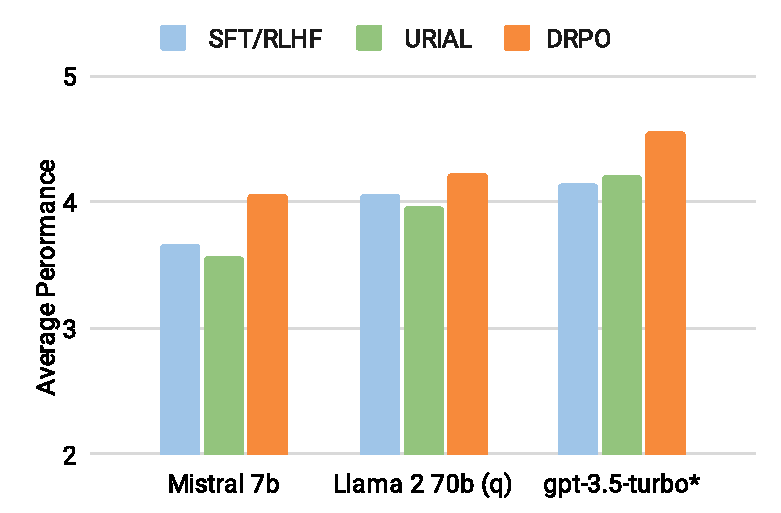
\includegraphics[width=1.0\linewidth]{images/method_comparison_column_chart_white_bg.pdf}
    \vspace{-15pt}
    \caption{与其他对齐方法(包括RLHF和URIAL~\cite{Lin2024ReAlign})的对比。 \ours在多个LLM上始终优于这两种基线。
    请注意,我们无法访问\texttt{gpt-3.5-turbo}基本模型;因此,\ours和URIAL直接应用于其RLHF调优版本。}
    \label{fig:overall_comparison_chart}
    \vspace{-15pt}
\end{figure}

\section{相关工作}
\vspace{-5pt}

\noindent \textbf{自对齐(Self-Alignment).}
传统的对齐方法严重依赖大量人工标注的偏好数据和通过强化学习训练的复杂奖励模型,这在可扩展性和成本方面带来了显著挑战~\cite{ouyang2022training}。自对齐关注的是利用模型生成的反馈、数据集、批判等手段对大语言模型自身进行对齐,然后用于微调或训练奖励模型~\cite{lee2023rlaif, bai2022training, cao2024towards, wang2024step, guo2024human}。典型的示例包括使用人类提供的指令和ICL示例合成对齐训练数据~\cite{wang2022self, kim2023aligning, sun2024principle},增强网页文档~\cite{li2023self},或自我批判机制~\cite{bai2022constitutional, madaan2024self}。然而,大多数这些方法仍然需要SFT/RLHF微调过程来增强对齐效果,同时也需要一定程度的人类标注或监督。相比之下,\ours 在使用自我批判错误反馈逐步对齐模型的原理上与自对齐方法类似,但它完全不依赖于任何模型微调或人工监督即可实现这一目标。

\begin{figure*}[ht]
    \centering
    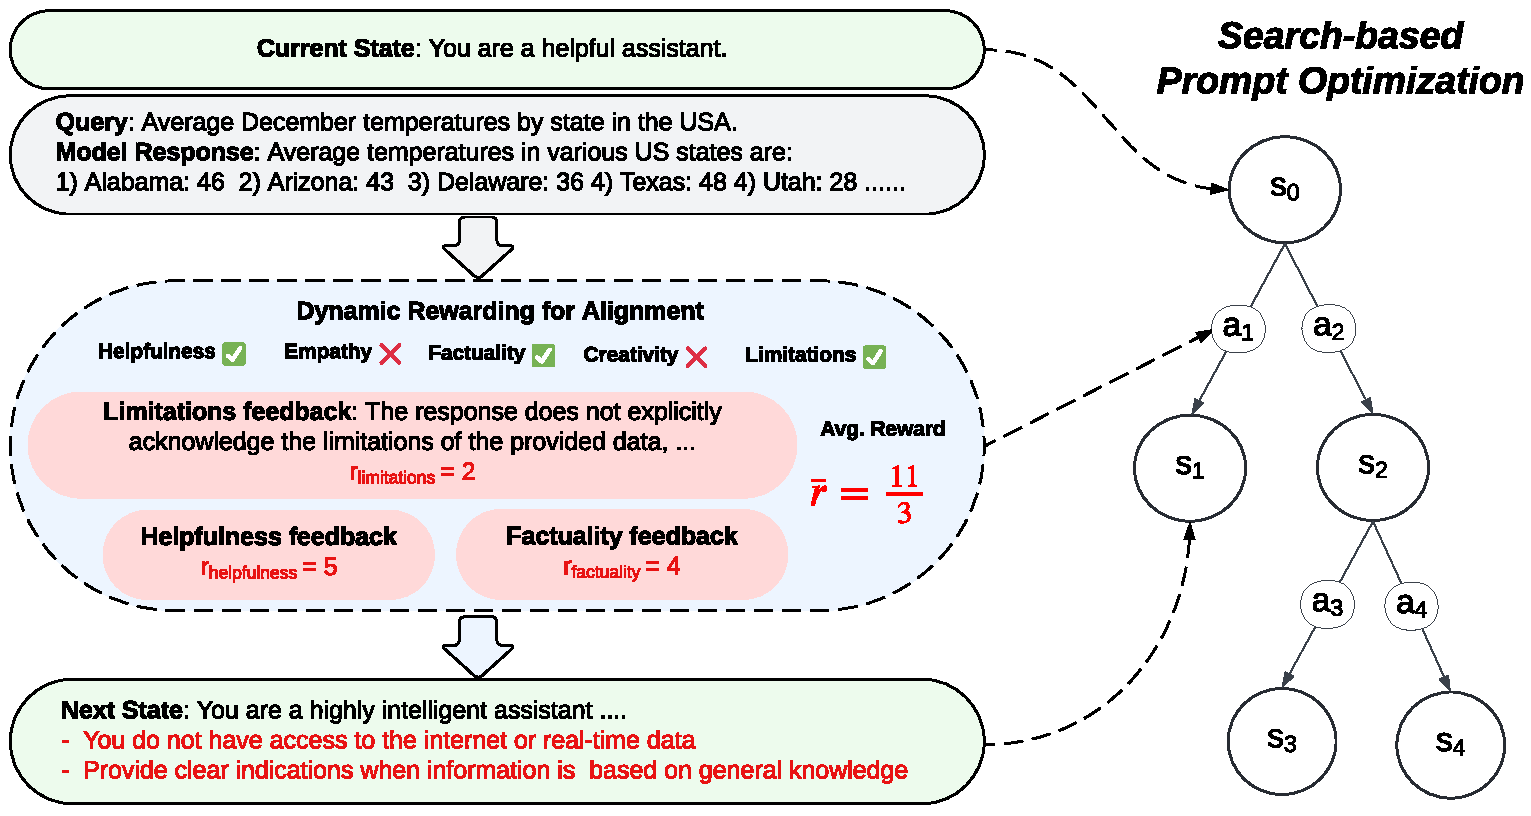
\includegraphics[width=0.95\linewidth]{images/Dynamic_Rewarding.pdf}
    \vspace{-8pt}
    \caption{带有提示优化的动态奖励整体框架(\ours)。该优化问题被建模为一个马尔可夫决策过程(MDP),并通过束搜索(beam search)求解以优化对齐提示。动态奖励作为该框架中集成的一项新技术,允许灵活分配奖励,以检测并解决当前大语言模型中的对齐弱点,从而增强整体优化过程。}
    \label{fig:dynamic_rewarding}
    \vspace{-15pt}
\end{figure*}

\noindent \textbf{免微调对齐(Tuning-Free Alignment).}
近年来,对齐研究的一个新趋势是无需更新参数来对齐大语言模型,通常作为训练后的处理步骤。当前主要有两类研究方向。第一类方法使用精心策划的人类标注和ICL示例进行模型对齐~\cite{han2023context, Lin2024ReAlign, zhao2024context};第二类方法则采用基于解码的策略,通过对齐奖励引导生成的token及其搜索过程~\cite{li2023rain, khanov2024args, huang2024deal}。虽然这些方法无需微调,第一类仍需人类策划,并且通常性能不及经过SFT/RLHF微调的模型;第二类虽然效果较好,但每次查询的推理成本较高,计算代价昂贵。值得一提的是,另一个有前景的方向是通过表示工程进行成本高效的对齐~\cite{zou2023representation, wu2024reft},该方法试图通过调整大语言模型的表示向量来实现对齐~\cite{li2024inference, kong2024aligning, wang2024inferaligner}。然而,这些方法并非真正意义上的免微调,通常仍需额外数据或模型训练来识别嵌入空间中的对齐方向。相比之下,\ours 无需任何额外标注或模型训练,仅需对每个模型进行一次性优化即可在性能上超过SFT/RLHF微调模型。

\noindent \textbf{提示优化(Prompt Optimization).}
发现最优的离散提示在当下变得尤为重要。现代大语言模型的提示通常分为两部分:上下文学习示例和详细指令。前者通常被视为一个检索问题,通过各种方案选择具有影响力的示例~\cite{rubin2021learning, dong2022survey}。而对后者的优化近来成为研究重点,通常被建模为一个采样或搜索问题。一般来说,会先提供一个初始提示(例如一个基本提示,“You are a helpful assistant”),然后启动一个迭代过程,在每一轮生成多样的提示候选,并保留最佳候选用于下一轮。为增加提示候选的多样性,研究提出了多种采样策略,例如反向翻译~\cite{xu2022gps}、进化操作~\cite{fernando2023promptbreeder}、自我批判~\cite{wang2023promptagent}。同时,也有多种搜索框架被提出,如蒙特卡洛搜索~\cite{zhou2022large}、进化算法~\cite{fernando2023promptbreeder, yang2023large}、束搜索~\cite{pryzant2023automatic}、以及蒙特卡洛树搜索(MCTS)~\cite{wang2023promptagent}。\ours 基于近年来的搜索优化方法,并引入动态奖励等新技术,有效应对对齐问题。

\section{Methodology}
\vspace{-5pt}


In this section, we introduce our formulation formally and present \ours for solving the alignment problem by optimizing the alignment instruction.

%Most existing methods for alignment use techniques like PPO \cite{Schulman2017ProximalPO} and DPO \cite{rafailov2023direct} which are very costly to execute as they need large amounts of data to be successful. 

% Most existing alignment methods, such as RLHF~\cite{ouyang2022training} and DPO~\cite{rafailov2023direct}, are generally expensive to execute, requiring not only large amounts of data but also substantial computational resources and human labeling efforts.
% Research on using in-context learning for alignment has been limited and primarily relies on human-generated prompts and in-context learning examples. To address this limitation, we introduce a systematic method to optimize prompts and in-context learning examples for LLMs without any human effort or annotation.


\subsection{Problem Formulation}

% \noindent \textbf{Problem Formulation}.
Given an LLM $\mathcal{B}$, an alignment instruction consists of two parts: a system prompt $\mathcal{P}$ and a set of $N$ in-context learning (ICL) examples $\mathcal{I}$.
The system prompt $\mathcal{P}$ serves as a prefix that provides high-level instructions, sets the tone, and imposes constraints on the model's responses. Each ICL example $\mathcal{I}_i$ consists of a pair $(q_i, d_i)$, where $q_i$ is an input query and $d_i$ is the corresponding desired response, so we can represent $\mathcal{I} = \{(q_1, d_1), (q_2, d_2), \ldots, (q_N, d_N)\}$. 

Conditioning on the system prompt $\mathcal{P}$ and a selected subset of $K$ ICL examples $\mathcal{I}_K \subseteq \mathcal{I}$, the aligned model response $y$ to an input $x$ is generated as:
\[
y = \mathcal{B}(x \mid \mathcal{P}, \mathcal{I}_K)
\]

\ours aims to optimize both system prompt $\mathcal{P}$ and ICL examples $\mathcal{I}_K$ to enhance alignment. This involves finding the best possible $\mathcal{P}^*$ and $\mathcal{I}_K^*$ that maximize the alignment of the model's responses. This optimization problem can be formulated as follows:
\[
(\mathcal{P}^*, \mathcal{I}_K^*) = \arg\max_{\mathcal{P}, \mathcal{I}_K} \mathbb{E}_{x \sim \mathcal{D}_x} \left[\mathcal{B}(x \mid \mathcal{P}, \mathcal{I}_K) \right]
\]
\noindent where $\mathcal{D}_x$ denotes the distribution of input queries, and the expectation $\mathbb{E}$ represents the alignment performance for responses based on specific metrics.


% We propose a two-step approach to the optimization problem: 
% \begin{enumerate}
%     \item Estimating $\mathcal{I}^*$ (universal).
%     \item Estimating $\mathcal{P}^*$ given ${\mathcal{I}}^*$. (model specific)
% \end{enumerate}


% \subsection{Systematic Optimization Framework}

% We approach the optimization of the system prompt $\mathcal{P}$ and in-context learning examples $\mathcal{E}$ using the unified framework LLM Reasoners~\cite{hao2024llm} that involves a base model $\mathcal{B}$, an optimizer $\mathcal{O}$, and an evaluator $\mathcal{E}$. This framework is treated as a search process that iteratively interacts with the model's environment and adjusts the prompt $\mathcal{P}$ based on a reward function $\mathcal{R}$. The main challenge for our problem is -the design of a reward function for a problem as broad and general as Alignment. To overcome this challenge we introduce `Dynamic Rewarding', which can effectively handle tasks as broad and challenging as alignment.


\subsection{Dynamic Rewarding with Prompt Optimization (\ours)}

Given the distinct nature of the system prompt and ICL examples, we propose to optimize them separately, resulting in a two-step optimization approach. We first construct a universal set of ICL examples and optimize their responses to obtain $\mathcal{I}^*$. Next, we estimate a model-specific system prompt $\mathcal{P}^*$ based on the optimized universal set $\mathcal{I}^*$. Notably, we leverage the \texttt{LLM Reasoners}\footnote{\url{https://github.com/maitrix-org/llm-reasoners}} framework~\cite{hao2023reasoning, hao2024llm} as the prompt optimization (PO) framework. Specifically, \texttt{LLM Reasoners} incorporates a base model $\mathcal{B}$, an optimizer $\mathcal{O}$, and an evaluator $\mathcal{E}$. It operates as a search agent that iteratively interacts with the model's environment, using the optimizer $\mathcal{O}$ to adjust the prompt $\mathcal{P}$ or ICL examples $\mathcal{I}$ based on a reward function $\mathcal{R}$. For further details, we refer readers to the original references. In the following, we introduce the core component of \ours. 


\subsubsection{Dynamic Rewarding for Alignment}

We formulate this optimization problem as a Markov Decision Process (MDP). In this framework, the states $s\in \mathcal{S}$ represent our optimization goal, which could be either a system prompt or an in-context example. Actions $a \in \mathcal{A}$ are defined based on the alignment feedback obtained during the evaluation of any given state. The key motivation is to leverage the superior generalization capabilities of LLMs to evaluate and analyze states, guiding state transitions toward an optimal state. We employ different evaluation techniques for system prompt and in-context example optimization, which are detailed in subsequent sections. Efficient traversal of this state space is crucial, and for this purpose, we adopt beam search due to its effectiveness and low computational cost.


One of the key challenges in our optimization task is designing a reward function capable of handling a problem as broad and generalized as alignment. As illustrated in Figure~\ref{fig:dynamic_rewarding}, a single, unified reward function is impractical due to the vast query space we aim to align with the base LLM $\mathcal{B}$. Different queries emphasize different focal points, meaning that certain evaluation criteria might be appropriate for some queries but not for others. To overcome this, we introduce a dynamic reward function $\mathcal{R}$, which can dynamically adapt to the specific query being evaluated. Notably, our approach shares conceptual similarities with a few recent alignment research, which also advocate for adaptable and query-sensitive alignment strategies~\cite{bai2022constitutional, sun2024principle}. However, the key distinction lies in our dynamic reward function’s ability to not only enable flexible evaluation but also integrate seamlessly into a formally defined optimization framework.



Specifically, we first predefined a set of reward criteria $\mathbb{R}$, from which the model dynamically selects the most relevant rewards, while also retaining the flexibility to propose new ones when necessary. Formally, for a given query \( q \), the dynamic reward function $\mathcal{R}$ evaluates the model's response $\sigma$ based on a dynamically selected or proposed rewards $\mathbb{R}_q$, where $\mathbb{R}_q \subseteq \mathbb{R} \cup \mathbb{R}^*$ and $\mathbb{R}^*$ represents newly proposed rewards. The reward function is defined as:

\[
\mathcal{R}(\sigma \mid \mathbb{R}_q) = \frac{1}{|\mathbb{R}_q|} \sum_{r \in \mathbb{R}_q} r(\sigma)
\]

Here, $\mathbb{R}_q$ denotes relevant rewards tailored for the given query \( q \) and \(r(\sigma)\) denotes the score of a specific reward when evaluating any response \(\sigma\). 

This allows us to flexibly score and evaluate responses based on the most relevant criteria for each specific query, ensuring that the evaluation remains contextually appropriate and comprehensive.




\subsubsection{ICL Example Optimization}

To optimize in-context learning examples, we start with a set of base ICL examples $\mathcal{I}_{\text{base}} = \{(q_1, b_1), (q_2, b_2), \ldots, (q_N, b_N)\} $, where $q_i$ is a query and $b_i$ is a base response to the query, $N$ is the total number of in-context examples. Our overall goal is to find a universal set $\mathcal{I}^{*}$ that maximizes alignment across various models.


We specifically optimize each ICL example $(q_i, b_i)$ individually. The initial state of the search tree for an ICL example is defined as the base response to the query, i.e.,  $s_0 = b_i$. At any time $t$, the state of the search tree, $s_t$, is the response of the example. This allows us to systematically monitor and evaluate the response at any given time $t$. The state space $\mathcal{S}$ encompasses all possible responses to the query $q_i$.


To evaluate and improve the alignment, we use the dynamic reward function $\mathcal{R}$. The relevant rewards $\mathbb{R}_{q_i}$ for the query $q_i$ are specifically selected or potentially proposed new rewards. The reward function $\mathcal{R}$ and evaluator $\mathcal{E}$ then evaluates the state $s_t$ based on these rewards, providing a reward $r_t$ and alignment feedback $a_t$:

\[
\begin{aligned}
& r_t = \mathcal{R}(s_t \mid \mathbb{R}_{q_i}) \\
& a_t = \mathcal{E}(s_t \mid \mathbb{R}_{q_i})
\end{aligned}
\]

Note that, in practice, evaluation and reward generation are performed simultaneously using one single prompt, so the evaluation can also be considered dynamic. The transition function $\mathcal{T}$, implemented by optimizer $\mathcal{O}$, then updates the state:
\[
s_{t+1} = \mathcal{T}(s_t, a_t)
\]

The detailed pseudo-code for this optimization process is provided in Algorithm \ref{alg:icl_opti} in Appendix \ref{sec:opti_algo} and the prompts used by our algorithm can be found in Appendix \ref{sec:meta_prompts}.



\subsubsection{System Prompt Optimization}

The optimization process for the system prompt is similar to that of the ICL example optimization. For the system prompt optimization, we use $K$ optimized ICL examples $\mathcal{I}_K^*  \subseteq \mathcal{I}^*$, where the $K$ ICL examples are chosen using similarity-based retrieval. We collect a set of seed samples $\mathcal{X} = \{x_1, x_2, \ldots, x_N \}$, where $x_i$ is a query that will be used to test the alignment of the base model $\mathcal{B}$. The goal of this process is to find the optimal prompt $\mathcal{P}^*$ (given that we already have access to $\mathcal{I}_K^*$), such that alignment of LLM $\mathcal{B}$ is maximized. This prompt is specific to the base model $\mathcal{B}$ and will provide the model with actionable insights and guidance to improve its alignment.


The optimization process begins by defining the initial state $s_0$ as the basic system prompt (e.g., ``You are a helpful assistant.''). At any time $t$, the state $s_t$ represents the current system prompt, and the state space $\mathcal{S}$ includes all possible system prompts for the given LLM $\mathcal{B}$.


For a given state $s_t$, we sample a query $x_t$ from the seed samples $\mathcal{X}$. The relevant rewards $\mathbb{R}_{x_t}$ for the query $x_t$ are specifically selected or potentially proposed new rewards. The reward function $\mathcal{R}$ and the evaluator $\mathcal{E}$ then evaluate the response generated by the model $\mathcal{B}$ given the system prompt $s_t$ and the selected in-context examples $\mathcal{I}_K^*$, providing a reward $r_t$ and alignment feedback $a_t$:

\[
\begin{aligned}
& r_t = \mathcal{R}(\mathcal{B}(x_t \mid s_t, \mathcal{I}_K^*)\mid \mathbb{R}_{x_t}) \\
& a_t = \mathcal{E}(\mathcal{B}(x_t \mid s_t, \mathcal{I}_K^*)\mid \mathbb{R}_{x_t})
\end{aligned}
\]

The optimizer $\mathcal{O}$ as a transition function then updates the state, $ s_{t+1} = \mathcal{T}(s_t, a_t) $. The detailed pseudo-code for this optimization process is provided in Algorithm \ref{alg:prompt_opti} in Appendix \ref{sec:opti_algo}.
\section{Experiments}


\subsection{Experimental Setup}


\begin{table*}[t]
\begin{center}
\begin{tabular}{ >{\raggedright\arraybackslash}p{3.9cm} c c c c c c c c }
    \toprule

    \textbf{[调整过的] 模型} & \textbf{方法} & \bm{$K$} & \textbf{有帮助} & \textbf{清晰} & \textbf{事实性} & \textbf{深度} & \textbf{参与度} & \textbf{平均} \\
    \midrule

    [\xmark] Mistral 7b  & 基础 & 0 & 2.20 & 2.51 & 2.29 & 1.69 & 1.80 & 2.10 \\

   [\xmark] Mistral 7b  & URIAL & 3 & 3.62 & 4.32 & 3.75 & 2.70 & 3.41 &  3.56\\

    [\xmark] Mistral 7b  & \ours & 2 & \textbf{4.23} & \textbf{4.56} & \textbf{3.97} & \textbf{3.68} & \textbf{3.84} &  \textbf{4.06}\\

    \hline

   [\cmark] Mistral 7b (Instruct) & 基础 & 0 & 3.98 & 4.44 & 3.64 & 2.97 & 3.26 &  3.66\\

   [\cmark] Mistral 7b (Instruct) & URIAL & 3 & 3.94 & 4.51 & 3.69 & 2.99 & 3.75 &  3.78\\

    [\cmark] Mistral 7b (Instruct) & \ours & 2 & \textbf{4.22} & \textbf{4.60} & \textbf{3.80} & \textbf{3.68} & \textbf{3.99} &  \textbf{4.06}\\

   \hline

    [\xmark] Llama 2 70b$^q$  & 基础 & 0 & 2.07 & 2.55 & 2.35 & 1.50 & 1.63 &  2.02 \\

    [\xmark] Llama 2 70b$^q$ & URIAL & 3 & 4.25 & 4.67 & 4.03 & 3.08 & 3.80 &  3.97 \\

    [\xmark] Llama 2 70b$^q$  & \ours & 2 & \textbf{4.42} & \textbf{4.72} & \textbf{4.23} & \textbf{3.81} & \textbf{3.98} &  \textbf{4.23}\\

    \hline

    [\cmark] Llama 2 70b$^q$ (chat) & 基础 & 0 & 4.36 & 4.71 & 3.95 & 3.56 & 3.76 &  4.07\\

    [\cmark] Llama 2 70b$^q$ (chat) & URIAL & 3 & 4.32 & 4.72 & 4.08 & 3.50 & 4.25 &  4.17\\

    [\cmark] Llama 2 70b$^q$ (chat) & \ours & 2 & \textbf{4.46} & \textbf{4.75} & \textbf{4.10} & \textbf{4.11} & \textbf{4.37} &  \textbf{4.36}\\

\hline

    [\xmark] Llama 3 8b  & 基础 & 0 & 1.82 & 2.27 & 2.20 & 1.38 & 1.48 &  1.83\\

    [\xmark] Llama 3 8b  & URIAL & 3 & 3.94 & \textbf{4.51} & 3.69 & 2.99 & \textbf{3.75} & 3.78 \\

    [\xmark] Llama 3 8b  & \ours & 2 & \textbf{4.02} & 4.40 & \textbf{3.84} & \textbf{3.50} & 3.65 &  \textbf{3.88} \\

   \hline

    [\cmark] Llama 3 8b (Instruct) & 基础 & 0 & 4.43 & 4.72 & 3.98 & 3.45 & 3.76 &  4.07\\

    [\cmark] Llama 3 8b (Instruct) & URIAL & 3 & 4.48 & 4.81 & \textbf{4.19} & 3.55 & 4.27 &  4.26\\

    [\cmark] Llama 3 8b (Instruct) & \ours & 2 & \textbf{4.54} & \textbf{4.81} & 4.16 & \textbf{4.08} & \textbf{4.40} & \textbf{4.40} \\

    \hline

    [\cmark] \texttt{gpt-3.5-turbo} & 基础 & 0 & 4.56 & 4.89 & 4.41 & 3.30 & 3.55 & 4.14 \\

    [\cmark] \texttt{gpt-3.5-turbo} & URIAL & 3 & 4.30 & 4.77 & 4.41 & 3.44 & 4.11 &  4.21\\

    [\cmark] \texttt{gpt-3.5-turbo} & \ours & 2 & \textbf{4.67} & \textbf{4.92} & \textbf{4.53} & \textbf{4.07} & \textbf{4.58} &  \textbf{4.55}\\

   \hline
    [\cmark] \texttt{gpt-4-0613} & 基础 & 0 & \textbf{4.71} & \textbf{4.93} & \textbf{4.52} & 3.49 & 3.53 &  \textbf{4.24} \\

    \bottomrule

\end{tabular}

\caption{在 \texttt{just-eval-instruct} 基准上的表现。``调整过的'' 表示该模型已进行 SFT/RLHF 调整。模型在多个方面进行评估:``有帮助''(帮助程度)、``清晰''(清晰度)、``事实性''(事实性)、``深度''(深度)和``参与度''(参与度)。基础方法表示基本的对齐提示。我们的方法在多个方面和整体上持续优于基础方法。}
\label{tab:main_table}
\vspace{-17pt}
\end{center}
\end{table*}



\noindent \textbf{Evaluation Dataset}.
We use the standard alignment benchmark, \texttt{just-eval-instruct}~\cite{Lin2024ReAlign}, which merges five popular alignment datasets to provide a comprehensive and fine-grained evaluation of LLM alignment. This benchmark consists of 1,000 examples: the first 800 assess the models' helpfulness, and the remaining 200 evaluate their harmlessness. The first 800 examples are evaluated based on five fine-grained aspects: \textit{helpfulness}, \textit{clarity}, \textit{factuality}, \textit{depth}, and \textit{engagement}, while the remaining 200 are evaluated using the \textit{safety} aspect. We use GPT-4 Turbo (\texttt{gpt-4-1106-preview}), one of the latest GPT-4 models available during our experiments, to evaluate both types of examples using the prompts specified in the original URIAL paper~\cite{Lin2024ReAlign}. The scoring scale ranges from 1 to 5, indicating ``strongly disagree'', ``disagree'', ``neutral'', ``agree'', and ``strongly agree''. Note that we employ a more recent version of GPT-4 compared to URIAL, which enhances the strictness and accuracy of our evaluation pipeline. Thus, we re-benchmark URIAL under our updated evaluation setting for consistency across all results.


\noindent \textbf{Seed Samples}. 
When optimizing the system prompt with \ours, we sample from our seed dataset $\mathcal{X}$ to measure the alignment performance of the system prompt at each time step. This seed dataset, consisting of 180 examples, is built using data from \texttt{AlpacaEval} \cite{alpaca_eval}, \texttt{LIMA} \cite{zhou2024lima}, and \texttt{HH-RLHF-redteam} \cite{Ganguli2022RedTL}. More details about the construction of this dataset can be found in Appendix \ref{sec:impl_details}.


\noindent \textbf{Models}.
We benchmark 6 open-source LLMs in our experiments: Mistral 7b (v0.1), Mistral 7b (Instruct)~\cite{Jiang2023Mistral7}, Llama 2 70$b^q$, Llama 2 70$b^q$ (chat) (4-bit AWQ~\cite{lin2023awq} quantized models)~\cite{Touvron2023Llama2O}, Llama 3 8b, Llama 3 8b (Instruct)~\cite{llama3modelcard} and 2 closed-source models: OpenAI's GPT-3.5 Turbo (\texttt{gpt-3.5-turbo}) and GPT-4 (\texttt{gpt-4-0613}). Models without the ``chat'' or ``instruct'' tag are base models, i.e., not tuned by SFT/RLHF. For evaluation, we use greedy decoding (temperature = 0) to ensure reproducibility.



\noindent \textbf{Baselines}. 
We first apply \ours to the base model, making the SFT/RLHF-tuned counterparts without \ours a natural baseline. For instance, we compare Mistral 7B + \ours and Mistral 7b (Instruct). Additionally, we have two more baselines: (1) The base method, where a basic prompt is applied without using ICL examples. (2) URIAL~\cite{Lin2024ReAlign}, where we use the prompt and ICL examples proposed by authors. We also provide extensive ablation baselines of our method, such as changing the search algorithm from Beam search to Greedy Search or Monte Carlo search and using ``static rewarding'' to understand the impact of dynamic rewarding. Full details of these can be found in Appendix~\ref{sec:impl_details}.




\noindent \textbf{Implementation details}.
We use GPT-4-turbo (\texttt{gpt-4-0125-preview}) as both the optimizer $\mathcal{O}$, and evaluator $\mathcal{E}$ unless specified otherwise. The initial set of in-context learning examples, $\mathcal{I}_{base}$, contains 16 examples: 3 from URIAL \cite{Lin2024ReAlign} and 13 generated using \texttt{gpt-4-0125-preview}. More details about the design choice made for $\mathcal{I}_{base}$ can be found in Appendix \ref{sec:impl_details}. We employ sentence transformers \cite{reimers-2019-sentence-bert} to retrieve K in-context learning examples from $\mathcal{I}^*$ given the query. We use $D$ as the beam depth, $W$ as the beam width, and $M$ as the number of action samples per state (to grow the tree for the next iteration). The exact hyper-parameters can be found in Appendix \ref{sec:impl_details}.


\subsection{Results}

\noindent \textbf{Comparison with baselines}. 
Table \ref{tab:main_table} presents the performance comparison of \ours with baselines. \ours outperforms all baselines across both tuned and un-tuned models. As shown in Figure \ref{fig:overall_comparison_chart} using \ours on strong base models such as Mistral 7b and LLama 2 70b$^q$ can surpass even the RLHF/SFT tuned models under base setting. It is noteworthy that \ours achieves superior performance compared to URIAL \citep{Lin2024ReAlign}, despite using fewer in-context learning examples, highlighting the quality of optimized alignment instruction by \ours. Note that while \texttt{just-eval-instruct} includes a \textit{safety} metric, we are not reporting it because, in our analysis, we found that the safety metric is saturated, with all methods (RLHF/SFT, URIAL, and \ours) achieving consistently high scores. This saturation is a good sign, demonstrating that tuning-free methods like \ours can result in very safe models that adhere to human values.



\noindent \textbf{Categorized performance}. 
Appendix~\ref{sec:cat_perf} presents the performance of models across various domains, e.g., ``procedure'', ``lifestyle'', ``info-seek'', ``STEM'', etc. In this experiment, we apply \ours to base models and compare their performance across multiple human-relevant and alignment-critical domains. \ours demonstrates consistently strong performance, surpassing RLHF/SFT-tuned models in most domains across all baselines.




\begin{table}[!t]
\begin{center}
\begin{tabular}{ c c c c }
    \toprule
    \multirow{2}{*}{\textbf{模型}} & \textbf{Mistral}  & \textbf{Llama}  & \textbf{基础} \\
    & \textbf{提示} & \textbf{提示} & \textbf{提示} \\
    \midrule
    Mistral 7b & \textbf{4.06} & 4.03 & 4.04 \\
    Llama 2 70$b^q$ & 4.19 & \textbf{4.23} & 4.17 \\
    \bottomrule
\end{tabular}
\caption{提示迁移对基础 LLM 的影响。针对目标基础 LLM 优化的提示可获得最佳性能。}
\label{tab:prompt_transfer}
\vspace{-17pt}
\end{center}
\end{table}

% Prompt Transfer table
\noindent \textbf{Prompt transfer}. 
We also conduct experiments on prompt transfer, i.e., evaluating the performance of an alignment instruction optimized for one LLM on a different LLM. Table~\ref{tab:prompt_transfer} presents the results of transferring various optimized prompts to Mistral 7b and Llama 2 70$b^q$. While the best results are achieved with prompts specifically optimized for the target model, transferring an optimized prompt can still lead to significant alignment improvements. This is evident in the case of LLaMA 2 70B$^q$, which benefits from the prompt optimized for Mistral 7B.





\noindent \textbf{Ablation on system prompt and  ICL examples}. 
Table \ref{tab:ablation_icl_prompt} shows the effect of ablating system prompt and in-context learning examples from \ours. Using both system prompt and in-context learning examples gave the best performance, underscoring the importance of both in alignment. It is worth pointing out that performance degradation on the removal of in-context learning examples was higher when compared to the removal of the system prompt, hinting that in-context learning examples are relatively important in alignment. Given this, our optimized in-context learning examples are a valuable asset and will be released publicly to facilitate further alignment research\footnote{\url{https://github.com/Singla17/DRPO}}.

\begin{table}[!t]
\begin{center}
\resizebox{0.9\linewidth}{!}{%
\begin{tabular}{ c c c c } 
 \toprule
 \multirow{2}{*}{\textbf{Model}} & \textbf{System} & \textbf{ICL} & \multirow{2}{*}{\textbf{Avg.}} \\
 & \textbf{Prompt} & \textbf{(}\bm{$K = 2$}\textbf{)} &  \\
 \midrule

  Mistral 7b  & \cmark & \cmark & \textbf{4.06} \\
 Mistral 7b (Instruct) & \cmark & \cmark & \textbf{4.06} \\
 Llama 2 70$b^q$  & \cmark & \cmark & \textbf{4.23} \\
 \texttt{gpt-3.5-turbo} & \cmark & \cmark & \textbf{4.55} \\

 \midrule


  Mistral 7b & \xmark & \cmark & 4.04 \\
 Mistral 7b (Instruct) & \xmark & \cmark & 4.04 \\
 Llama 2 70$b^q$  & \xmark & \cmark & 4.17 \\
 \texttt{gpt-3.5-turbo} & \xmark & \cmark & 4.42 \\

  \midrule


 Mistral 7b (Instruct) & \cmark & \xmark & 3.67 \\
 Llama 2 70$b^q$  & \cmark & \xmark & 3.63 \\
 \texttt{gpt-3.5-turbo} & \cmark & \xmark & 4.34 \\

  \bottomrule

\end{tabular}
}
\caption{Ablation study on the impact of removing the optimized system prompt and in-context learning (ICL) examples optimized using our method. In the absence of the optimized system prompt, a basic system prompt is provided. Our method consistently outperforms all ablation variants across all models.}
\label{tab:ablation_icl_prompt}
\vspace{-20pt}
\end{center}
\end{table}


% Search Algo Ablation table
\noindent \textbf{Ablation on search algorithms}. 
Table \ref{tab:ablation_search_algo} presents the effect of search algorithms on prompt optimization. We have kept the state and action definitions the same and have only changed the underlying search algorithm.  In this experiment, we ensured that MC and Beam sample the same number of prompts, i.e., same cost, whereas greedy search has a lower cost because the beam width is fixed at 1. More implementation details can be found in Appendix \ref{sec:impl_details}. \ours with beam search gives the best results, depicting the need for thoughtful search and efficient optimization for optimal results.

\begin{table}[!t]
\begin{center}

\begin{tabular}{ c c c  } 
    \toprule
    \textbf{Model} & \textbf{Search} & \textbf{Avg.} \\
    % \multirow{2}{*}{Model} & Prompt &  \multirow{2}{*}{Avg.} \\
    % & Search &  \\
    
    \midrule
    Mistral 7b (Instruct) & Beam  & \textbf{4.06} \\
    \midrule
    
    Mistral 7b (Instruct) &  MC  & 4.02 \\
    Mistral 7b (Instruct) & Greedy & 4.02 \\
    
    \bottomrule
    
\end{tabular}

\caption{Ablation study on search methods. MC: Monte Carlo Search; Greedy: greedy search; Beam: beam search. Our method outperforms all other search algorithms tested in the ablation study.}
\vspace{-10pt}
\label{tab:ablation_search_algo}
\end{center}
\end{table}




% Methodological Ablation table

\begin{table}[!t]
\begin{center}
\resizebox{0.9\linewidth}{!}{
\begin{tabular}{ c c c c }
    \toprule
    \multirow{3}{*}{\textbf{模型}} & \textbf{动态} &  \textbf{动态}  &\multirow{3}{*}{\textbf{平均}} \\
    & \textbf{奖励} &  \textbf{奖励 } \\
    & \textbf{提示} & \textbf{ICL} \\

    \midrule
    Mistral 7b (指令) & \cmark  & \cmark & \textbf{4.06} \\
    \midrule

    Mistral 7b (指令) &  \xmark  & \cmark  & 4.02 \\
    Mistral 7b (指令) & \cmark & \xmark & 3.86 \\

    \bottomrule

\end{tabular}}

\caption{关于动态奖励的消融研究,检查其从系统提示和 ICL 示例优化中去除的影响。我们的方法,通过对提示和 ICL 示例使用动态奖励,始终优于两种消融变体。}
\label{tab:ablation_method}
\end{center}
\vspace{-20pt}
\end{table}



\noindent \textbf{Ablation on dynamic rewarding}.
We performed ablations on the dynamic rewarding mechanism. Table \ref{tab:ablation_method} depicts that \ours, with its current setting of using dynamic rewards for system prompt and ICL optimization, works the best. The in-context examples and prompts without using Dynamic rewarding are also optimized by `static rewarding' for a fair comparison, i.e., we ask the Optimizer to optimize all the rewards all the time. More details can be found in Appendix \ref{sec:impl_details}. 



\noindent \textbf{Effect of the number of in-context examples}.
Figure \ref{fig:icl_variation_chart} visualizes the effect of changing the number of in-context learning examples on alignment performance. The choice of $K = 2$ resulted in the best overall performance for Mistral 7b, ensuring strong alignment at a lower context length cost. Also, as observed in Figure \ref{fig:icl_variation_chart}, higher $K$ does not necessarily improve performance, hinting that the quality of ICL examples is more important. The importance of quality is also highlighted in Table \ref{tab:main_table}, where \ours outperforms URIAL at a lower $K$.


% ICL variation line chart
\begin{figure}[!t]
    \centering
    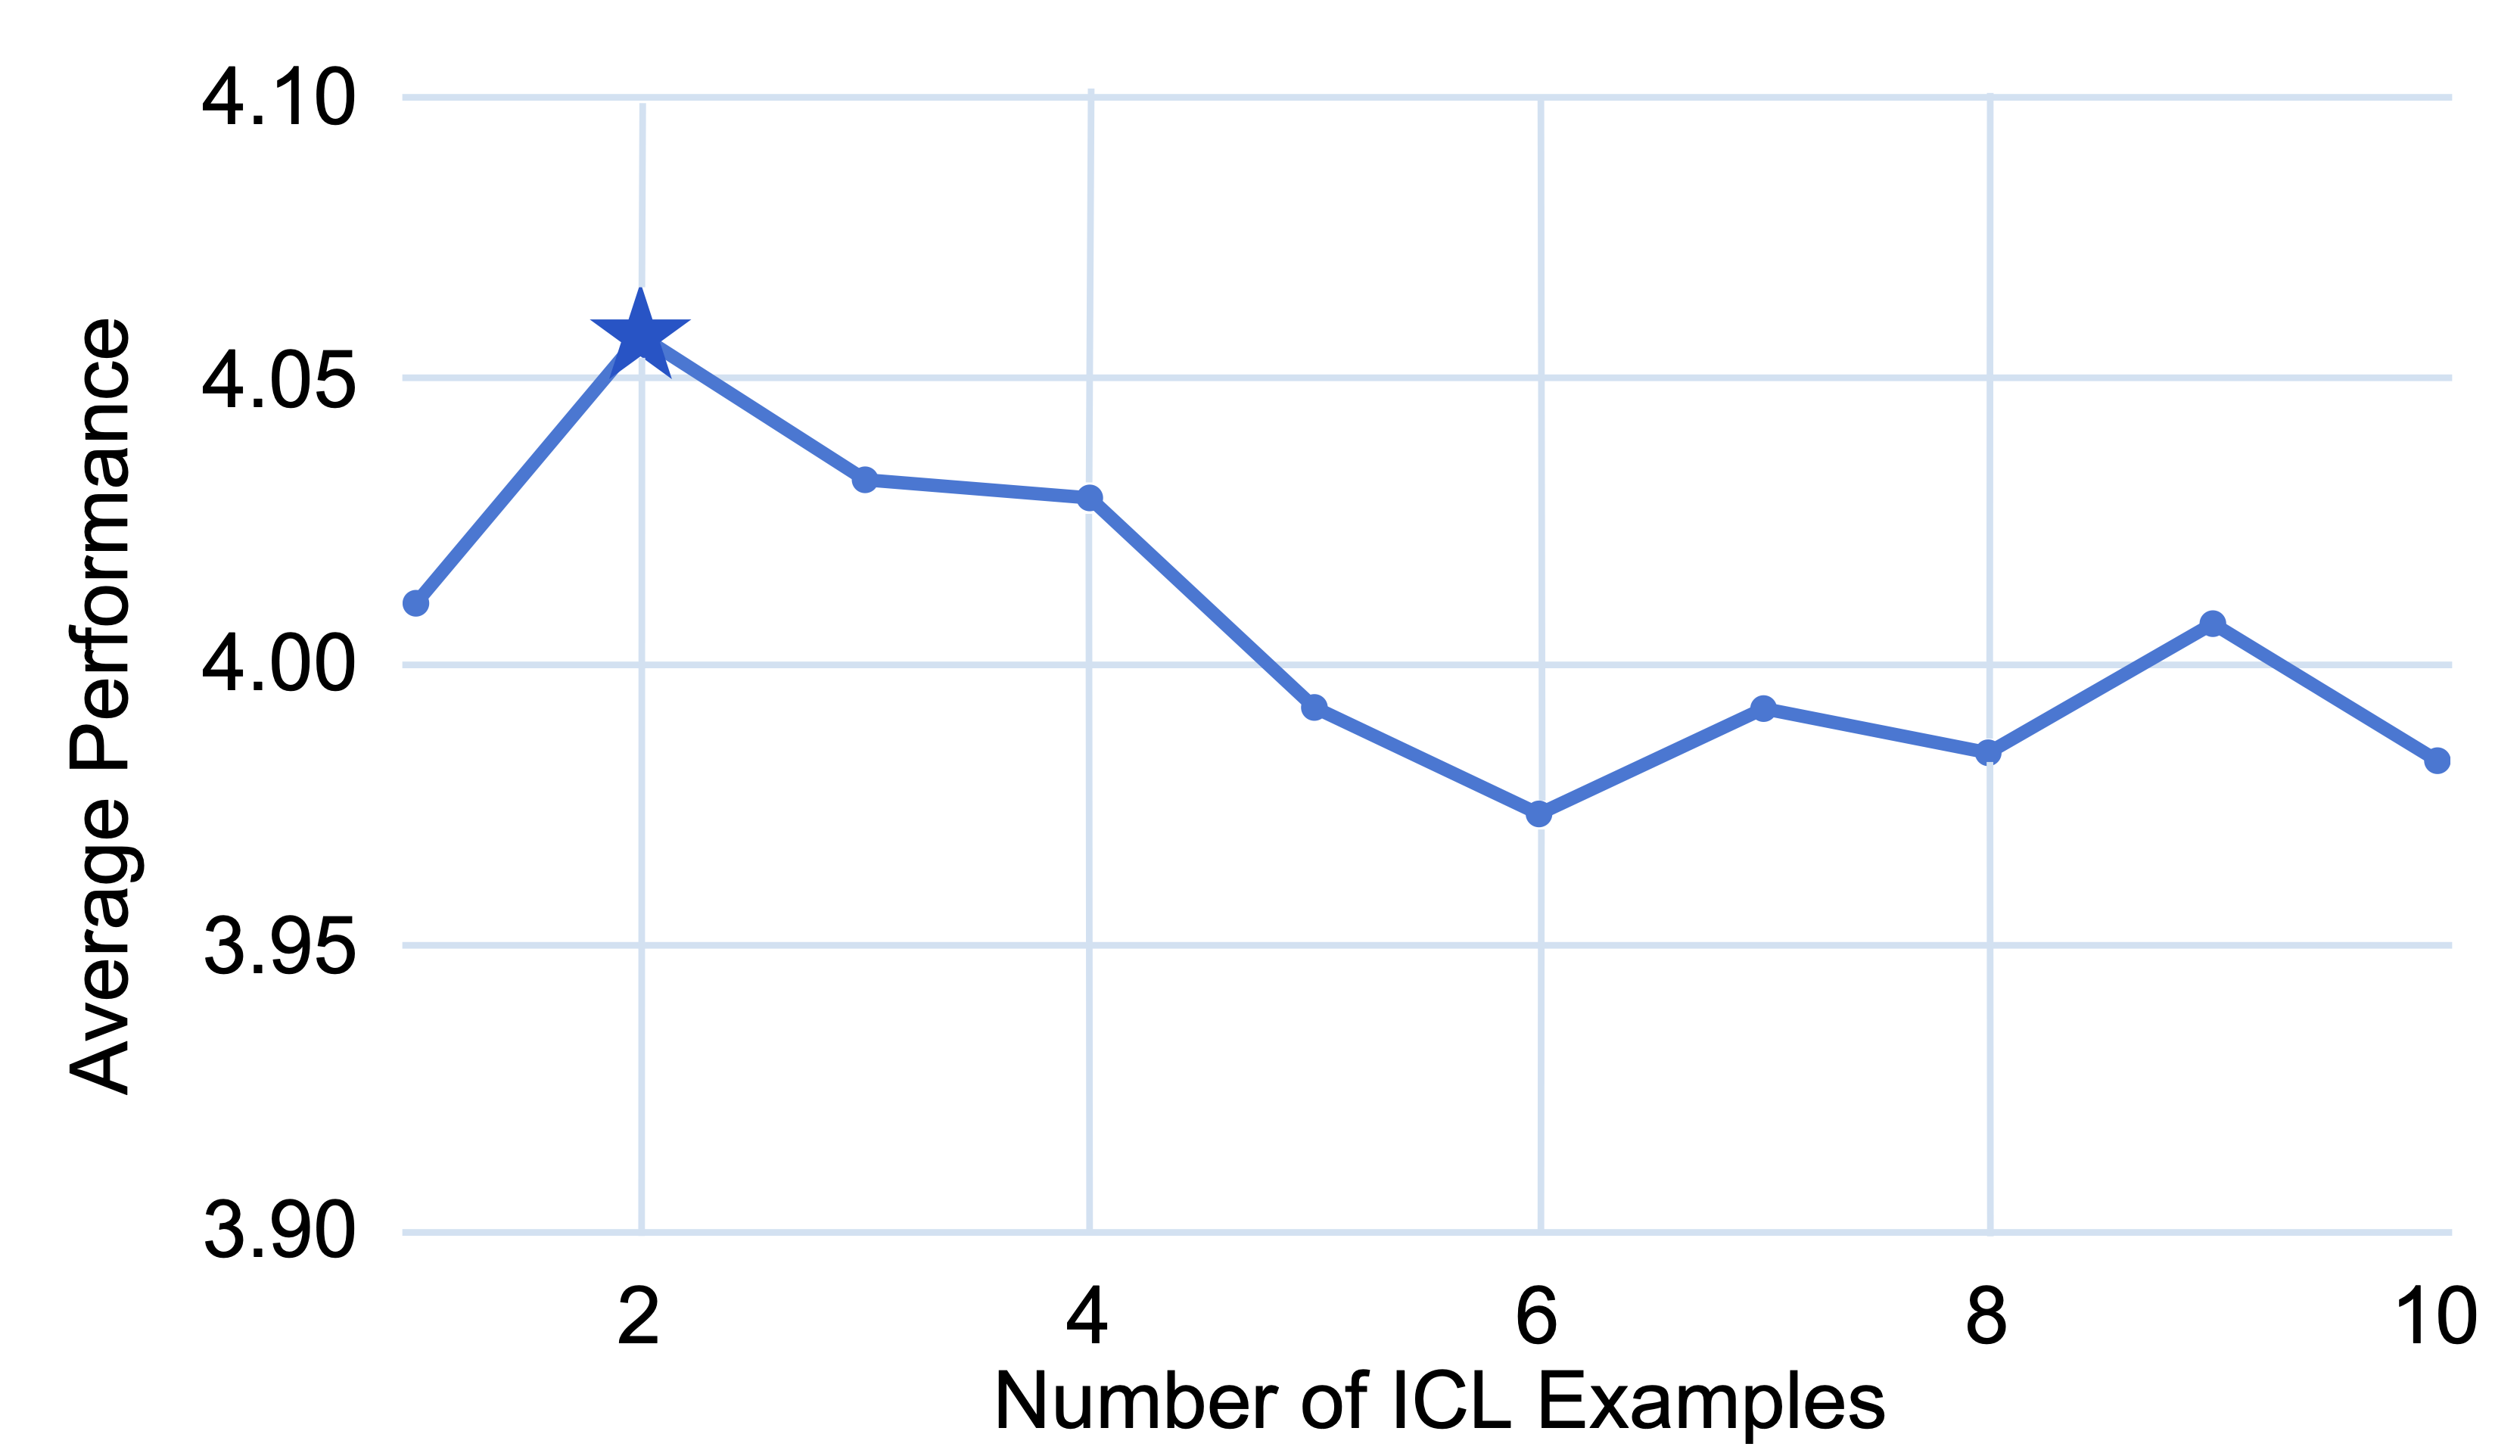
\includegraphics[ width=\linewidth]{images/icl_variation_line_chart_white_bg_v2.png}
    \caption{Performance of Mistral 7b (Instruct)  on varying the number of ICL examples. Two examples give us the best performance with a lower context length cost.}
    \label{fig:icl_variation_chart}
    \vspace{-5pt}
\end{figure}



% Qualitative analysis of gpt prompt
\newcommand{\reduline}[1]{{\color{red}\underline{{\color{black}#1}}}}

\newcommand\dunderline[2][.2pt]{\raisebox{-#1}{\underline{\raisebox{#1}{\smash{\underline{#2}}}}}}

\begin{table}[!t]

\definecolor{Gray}{gray}{0.90}
\newcolumntype{a}{>{\columncolor{Gray}}c}
\centering
\resizebox{1\linewidth}{!}{
\begin{tabular}{@{}p{10cm}@{}}
\toprule
\textbf{优化的对齐提示} \\
\midrule
作为一个有帮助且道德的助手,您的主要目标是提供准确、引人入胜、清晰和情感共鸣的回应,涵盖广泛的查询。 \\
- \ctext[RGB]{230,246,255}{努力使复杂话题变得易于理解且富有情感共鸣,以人类般和易于理解的方式进行沟通。组织您的回应以增强可读性和情感联系,避免过多的技术性术语。}  \\
- \ctext[RGB]{233,252,232}{始终承认您知识的局限性,特别是在推测历史“假设”、未来预测或解释情感时。} \\
- \ctext[RGB]{255,225,255}{力求在详细的信息内容与对话性、引人入胜的语气之间找到平衡。结合故事性元素、例子、类比和直接提问,使信息更具可关联性。} \\
- \ctext[RGB]{230,246,255}{避免给用户提供过多信息;构建清晰、组织良好的回应,考虑到用户的认知负担。}
 \\

 \bottomrule
\end{tabular}
}

\caption{针对 \texttt{gpt-3.5-turbo} 优化的系统提示片段。优化后的提示清晰地展示了改进的对齐,解决了模型的潜在弱点。}
\label{tab:gpt_prompt}
\vspace{-15pt}
\end{table}

\noindent \textbf{Qualitative analysis of optimized prompts}. 
We finally present qualitative results to show \ours' ability to identify a model's alignment weaknesses and tailor system prompts to address them, as shown in Table \ref{tab:gpt_prompt} for \texttt{gpt-3.5-turbo}. The color-coded text in the table highlights specific weaknesses of \texttt{gpt-3.5-turbo} identified by \ours, along with actionable insights. Notably, it highlights \ctext[RGB]{233,252,232}{knowledge limitations of the model}, \ctext[RGB]{255,225,255}{tips to improve engagement} and \ctext[RGB]{230,246,255}{technical verbiage}. For a weaker model like Mistral 7b, \ours identifies the problem of repetitive tokens, which is absent in a strong model like \texttt{gpt-3.5-turbo}. Complete optimized prompts for both models, along with detailed annotations on the differences, can be found in Appendix \ref{sec:prompt_case_study}.  

% radar chart, analyzing various domains/dimensions 

\vspace{-5pt}
\section{结论}
\vspace{-5pt}

本文提出了动态奖励与提示优化相结合的方法(\ours),这是一种无需微调即可实现大语言模型自我对齐的策略。\ours 将一种新颖的动态奖励机制融入基于搜索的提示优化框架,使大语言模型能够自适应地改进其特定的对齐弱点。对八个大语言模型的实验表明,经过 \ours 增强的基础模型在性能上优于经过 SFT/RLHF 微调的同类模型,其优化后的提示也超过了人类专家所设计的提示。\ours 的适应性与高效性为构建更加个性化的人工智能系统提供了一条有前景的路径。

\newpage
\section*{局限性}

尽管 \ours 在无需调优的自我对齐方面展示了显著的进展,但仍有一些潜在的局限性需要讨论。

\noindent \textbf{优化成本。}  
无需调优的对齐并非不付出代价。理想情况下,为每个查询优化对齐提示可能会更有效,但其计算开销是不可接受的。这个问题类似于基于解码的对齐,其中对齐引导的解码需要针对每个查询进行。然而,\ours 只需要对每个 LLM 进行一次优化,从而将优化后的对齐提示存储在 LLM 内存中供以后使用,显著减少了开销。关于 \ours 的成本的详细分析可以在 \ref{sec:i_cost} 中找到。

\noindent \textbf{计算开销。}  
与 SFT / RLHF 调优的模型相比,\ours 中优化和复杂提示所增加的输入上下文引入了微小的计算开销。随着现代 LLM 的发展,例如更大的上下文窗口,我们认为这种计算开销是可以管理的。此外,一旦有了优化提示,\ours 可以通过提示压缩技术进一步减少提示的长度,而不会牺牲性能,未来的工作可以进一步探讨这一点。

\noindent \textbf{自动奖励。}  
另一个我们注意到的潜在局限性是 \ours 中完全自动化的内部奖励过程可能被忽视。例如,动态奖励可能会分配不精确的奖励,导致不良行为。我们承认这一潜在问题,并已经手动审查了优化提示,未发现与此自动化优化过程相关的严重问题。未来的工作应该开发系统化的方法来监控并确保奖励分配的准确性以及由此产生的模型行为。

\noindent \textbf{LLM 的自我修正能力。}  
LLM 的自我修正能力也可能是一个潜在的局限性。在优化系统提示和上下文示例时,我们依赖于 LLM 生成的反馈,而这些反馈有时可能是不准确的。在分析反馈痕迹时,我们观察到虽然一些反馈过于苛刻,但大多数反馈是建设性的。重要的是,搜索过程减轻了过于苛刻或不正确的反馈对整体优化质量的影响。未来的工作可能会探索额外的保护措施,以进一步确保 LLM 生成的反馈在整个过程中是正确和可靠的。

\noindent \textbf{与微调的结合。}  
人们可能自然会想知道,\ours 是否可以用来合成对齐数据,并与微调方法结合以进一步提高对齐性能。答案是肯定的;然而,正如论文中所强调的,\ours 的独特优势之一是其适应性,能够迅速适应新的奖励或用户特定的要求。我们重视这种特性,并将 \ours 与微调的结合留待未来的工作进行探讨。

\noindent \textbf{模型的容量假设。}  
\ours 所涉及的模型有一些假设。首先,\ours 利用强大的 LLM,特别是 GPT-4,作为优化器来最大化动态奖励和对齐反馈的性能。未来的研究可以探索其他优化器模型,包括开源选项,从而实现 \ours 的应用普及。此外,\ours 对基础模型提出了一定的容量要求。考虑到我们优化的对齐提示的复杂性,较小且不太强大的 LLM,如 LLaMA-7b~\cite{touvron2023llama},可能无法通过 \ours 获得显著的提升,尽管仍然可能有一定的增强。我们的假设是,经过更好预训练和能遵循指令的模型有更大的潜力通过 \ours 得到增强。我们将这个有意义的问题留给未来的研究,探索 LLM 的对齐潜力和阈值。

最后,未来的工作可能会进一步探索动态奖励机制的增强和 \ours 在不同领域和任务中的更广泛应用。
\section*{致谢}

我们感谢匿名评审人提供的建设性评论和建议。我们还感谢 Enze Ma 将 \ours 集成到 \texttt{LLM Reasoners} 中,并感谢与 MixLab 成员的宝贵讨论。本研究得到了 OpenAI Agentic AI 研究资助计划的支持。本文中表达的观点和结论仅代表作者本人,未必反映资助机构的观点。



% \section*{Acknowledgments}

% This document has been adapted
% by Steven Bethard, Ryan Cotterell and Rui Yan
% from the instructions for earlier ACL and NAACL proceedings, including those for
% ACL 2019 by Douwe Kiela and Ivan Vuli\'{c},
% NAACL 2019 by Stephanie Lukin and Alla Roskovskaya,
% ACL 2018 by Shay Cohen, Kevin Gimpel, and Wei Lu,
% NAACL 2018 by Margaret Mitchell and Stephanie Lukin,
% Bib\TeX{} suggestions for (NA)ACL 2017/2018 from Jason Eisner,
% ACL 2017 by Dan Gildea and Min-Yen Kan,
% NAACL 2017 by Margaret Mitchell,
% ACL 2012 by Maggie Li and Michael White,
% ACL 2010 by Jing-Shin Chang and Philipp Koehn,
% ACL 2008 by Johanna D. Moore, Simone Teufel, James Allan, and Sadaoki Furui,
% ACL 2005 by Hwee Tou Ng and Kemal Oflazer,
% ACL 2002 by Eugene Charniak and Dekang Lin,
% and earlier ACL and EACL formats written by several people, including
% John Chen, Henry S. Thompson and Donald Walker.
% Additional elements were taken from the formatting instructions of the \emph{International Joint Conference on Artificial Intelligence} and the \emph{Conference on Computer Vision and Pattern Recognition}.

% Bibliography entries for the entire Anthology, followed by custom entries
%\bibliography{anthology,custom}
% Custom bibliography entries only
\bibliography{main}

\appendix

\newpage


\section{更多实现细节}
\label{sec:impl_details}
\subsection{ \ours 的超参数}
\begin{table}[H]
\begin{center}
\begin{tabular}{ c c c c }
    \toprule
    \textbf{实验} & \bm{$W$} & \bm{$M$} & \bm{$D$} \\
    \midrule
    ICL 优化 & 1 & 1 & 5 \\
    系统提示优化 & 2 & 3 & 20 \\
    \bottomrule
\end{tabular}
\caption{\ours 在 ICL 优化和系统提示优化过程中使用的所有超参数。}
\end{center}
\label{tab:hyper_params_beam}
\end{table}

\subsection{基准}

\noindent \textbf{蒙特卡罗搜索}:蒙特卡罗搜索执行无方向的单步采样多次。采样方法与\ours相同;我们在该方法中采样了120个提示,以确保与\ours的成本相同,从而保证公平比较。

\noindent \textbf{贪心搜索}:贪心搜索是束搜索的特例,其中束宽度$W$固定为1,采样方法、每个状态的动作样本数$M$与\ours保持一致,但由于该方法中的束宽度减少,整体成本较低。

\noindent \textbf{静态奖励}:在此方法中,我们保持与\ours相同的搜索算法。不同的是,我们总是向优化器和评估器提供一组固定的评估方面,而不是选择动态方面。固定的评估方面包括有用性、清晰度、事实性、深度、参与度和安全性,即评估方面。这使得静态奖励方法在评估指标上表现最佳,并建立了一个强有力的基准。请注意,在评估此基准时,我们保持了2个上下文学习示例的数量。
\subsection{种子样本}
在采样数据集中,180个样本中,$47.8 \%$ 的样本来自 \texttt{AlpacaEval},$28.9 \%$ 来自 LIMA,其余来自 \texttt{HH-RLHF-redteam}。我们通过仅采样那些不在评估数据集中的示例,确保了公平的评估。
\subsection{基础 ICL 示例}  
\label{sec:i_base}  
$\mathcal{I}_{base}$ 中的示例被分为两类:“不道德的”,用于训练模型应对恶意查询;以及“信息性的”,用于训练模型以可接受的格式呈现相关信息。$\mathcal{I}_{base}$ 包含数量相等的“不道德”查询和“信息性”查询。
\subsection{ \ours 的成本分析}
\label{sec:i_cost}
\noindent \textbf{系统提示优化}。
我们的优化过程采用了束搜索策略,采样提示的数量由参数 $W$(束宽度)、$M$(每个状态的动作样本数)和 $D$(束深度)决定。具体来说,这些参数导致:

    \begin{enumerate}
        \item  $W \times M \times D$ 次 API 调用优化器 LLM $\mathcal{O}$ 进行提示采样。
        \item $D$ 次 API 调用 LLM 进行种子样本的奖励选择。
        \item $W \times M \times D$ 次 API 调用基础 LLM $\mathcal{B}$ 生成与每个采样提示对应的响应。
        \item $W \times M \times D$ 次 API 调用评估器 LLM $\mathcal{E}$,使用种子样本评估采样提示。
    \end{enumerate}

因此,系统提示优化的总体成本($C_{\text{system}}$),包括 API 调用和基础 LLM 推理,可以表示为:

\begin{align*}
    C_{\text{system}} = & \underbrace{W \times M \times D}_{\text{提示采样}}
    + \underbrace{D}_{\text{奖励选择}} + \\
    & \underbrace{W \times M \times D}_{\text{响应生成}}
    + \underbrace{W \times M \times D}_{\text{提示评估}}
\end{align*}

值得注意的是,奖励选择成本仅发生一次,因为这些结果会被缓存并在所有模型中重复使用。此外,系统提示优化对于每个模型也是一次性过程;一旦优化完成,提示可以在不产生额外成本的情况下重复使用。这种方法确保了所产生的成本是有限的,并且不会随着后续使用次数的增加而扩大。

\noindent \textbf{ICL 优化}。
与系统提示优化类似,我们也可以使用束搜索进行 ICL 优化。优化一个 ICL 示例的成本如下:

    \begin{enumerate}
        \item 单次 API 调用 LLM 进行示例的奖励选择。
        \item $W \times M \times D$ 次 API 调用评估器 LLM 评估 ICL 示例。(根据超参数,结果为 5)
        \item $W \times M \times D$ 次 API 调用优化器 LLM,优化 ICL 示例。
    \end{enumerate}

因此,ICL 优化的总成本($C_{\text{ICL}}$)可以表示为:

\begin{align*}
    C_{\text{ICL}} = \quad & (\underbrace{1}_{\text{奖励选择}} + \underbrace{W \times M \times D}_{\text{评估}} + \\
    & \underbrace{W \times M \times D}_{\text{优化}} ) \times N
\end{align*}

其中 $N$ 表示我们希望优化的示例数量。

ICL 示例是与模型无关的,可以在不同模型之间重复使用,因此使得优化成本对于每个示例来说是一次性支出。

\newpage


\section{分类性能}
\label{sec:cat_perf}
\subsection{Mistral 7b}
\begin{figure}[h]
\centering
\begin{subfigure}[b]{.5\textwidth}
  \centering
  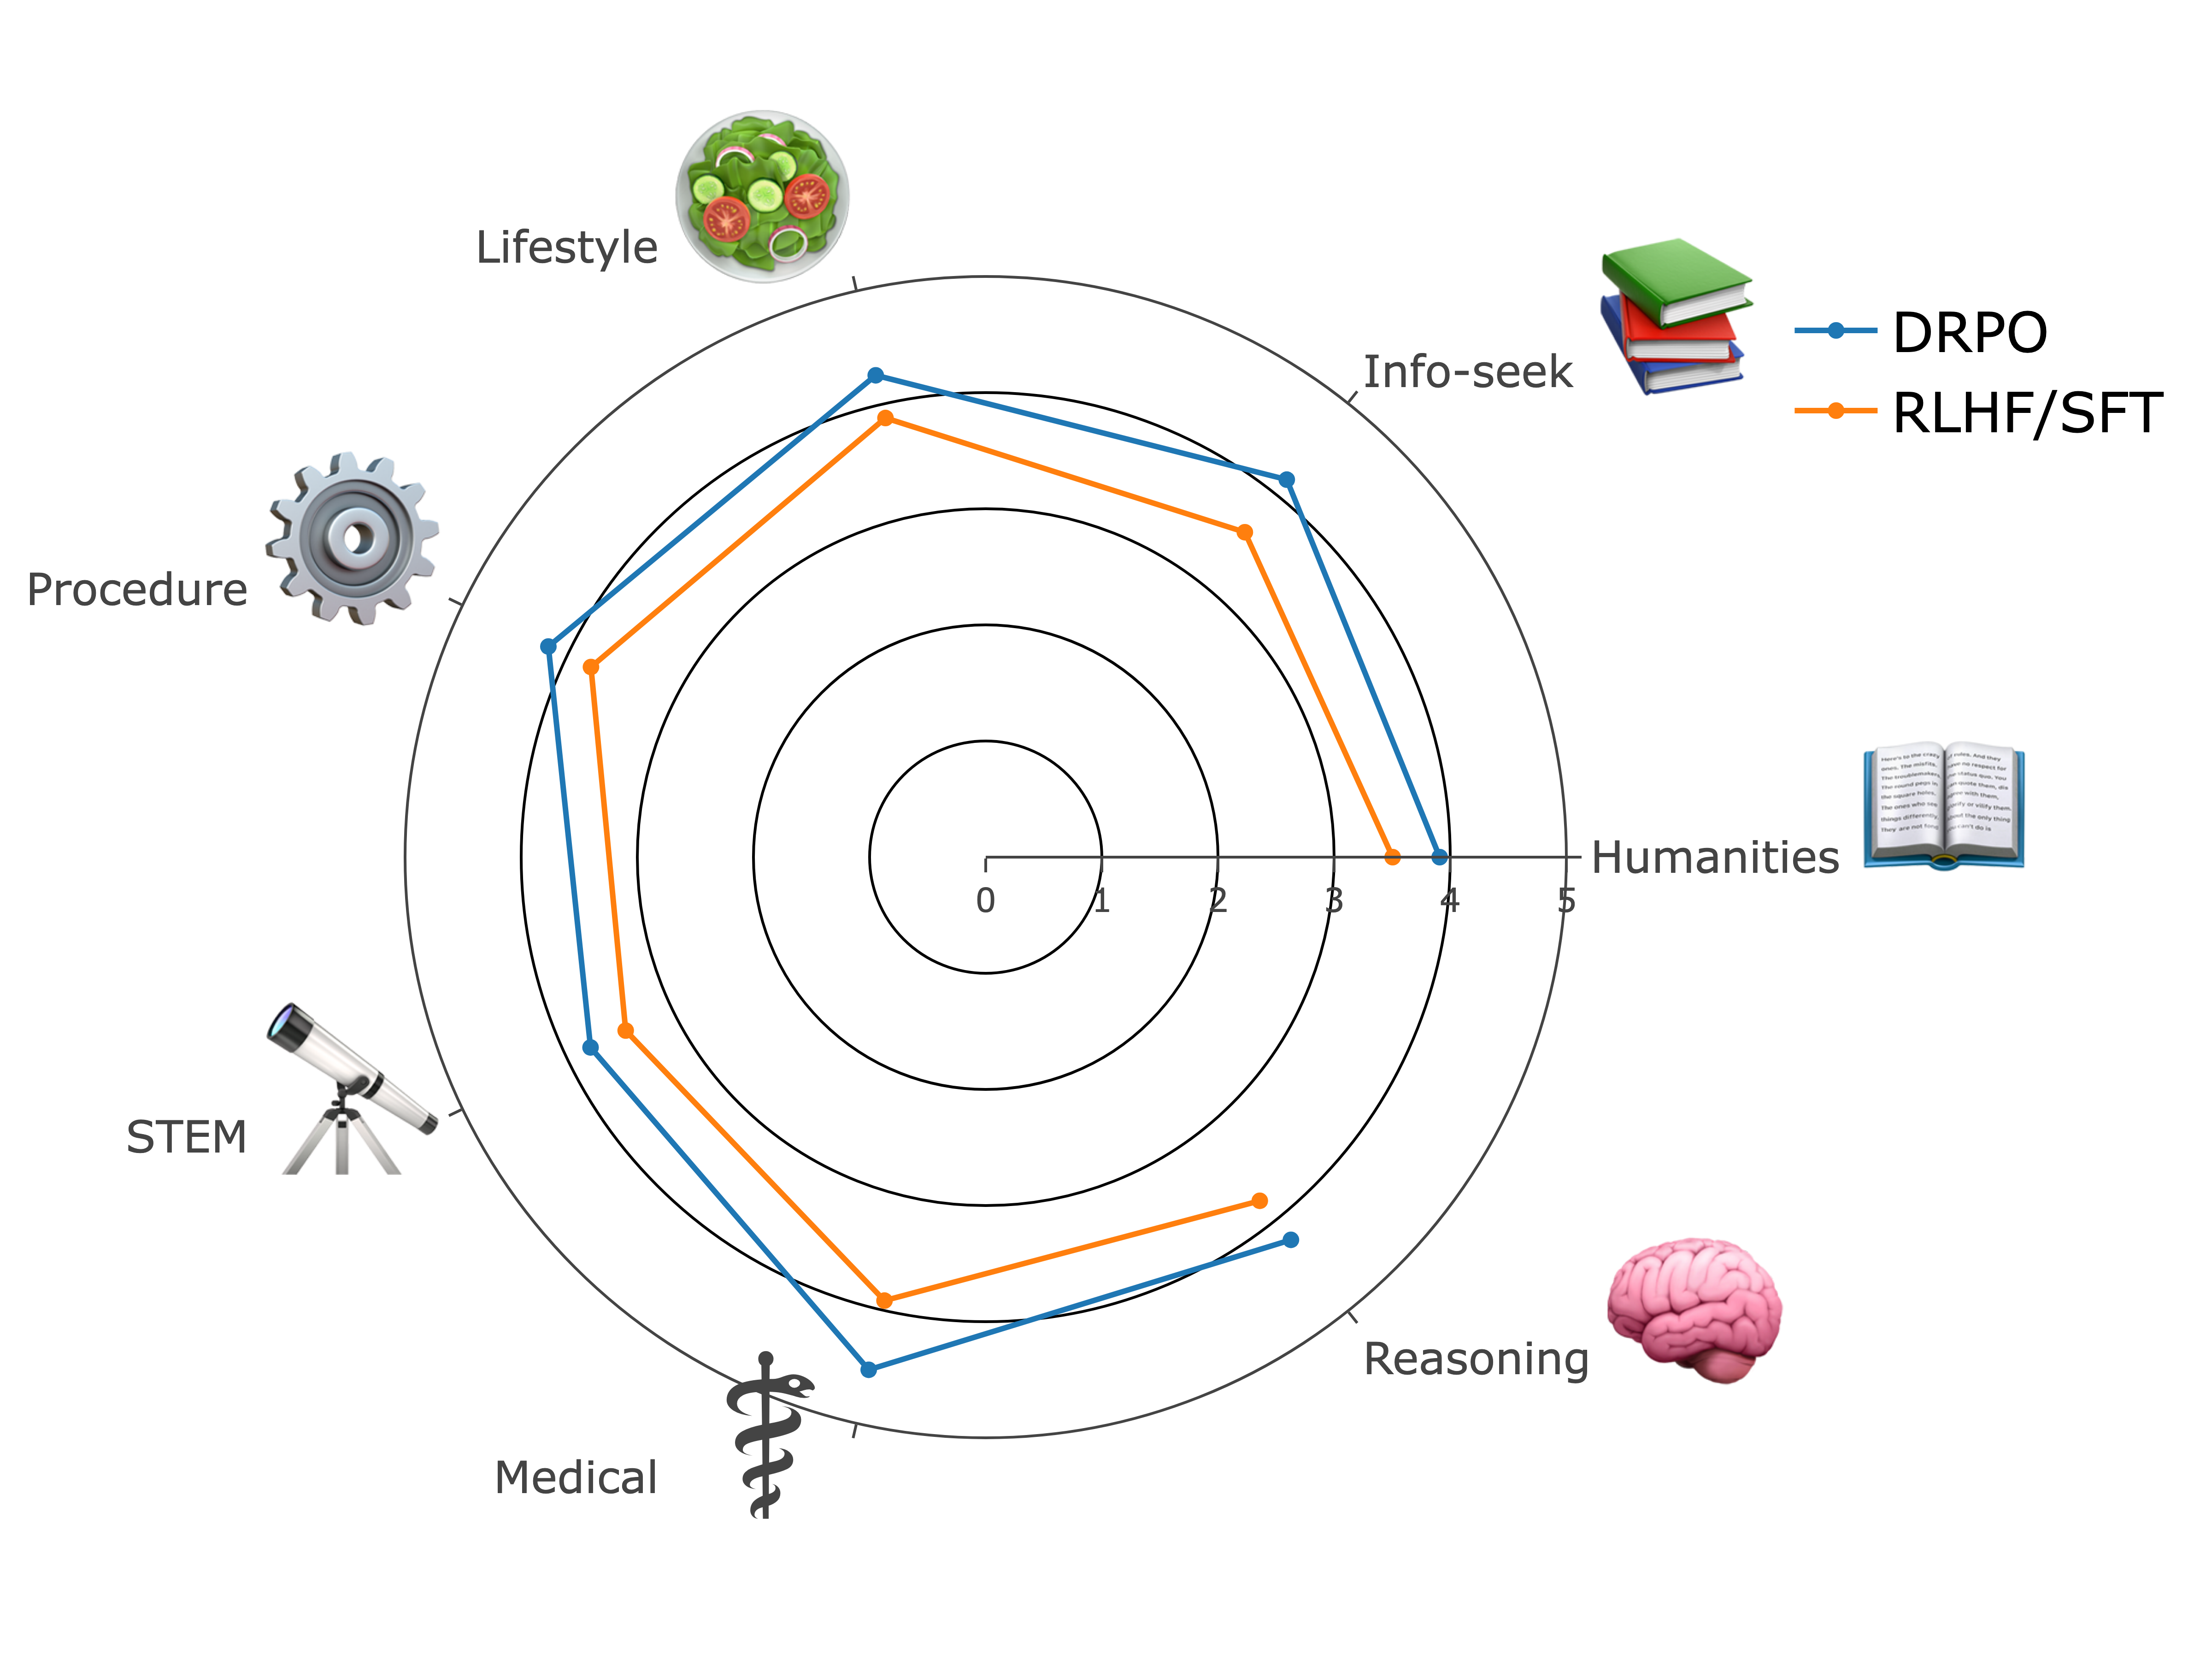
\includegraphics[width=0.95\linewidth]{images/mistral_1.png}
  \label{fig:cat_mistral_1}
\end{subfigure}

\vspace{1em}

\begin{subfigure}[b]{.5\textwidth}
  \centering
  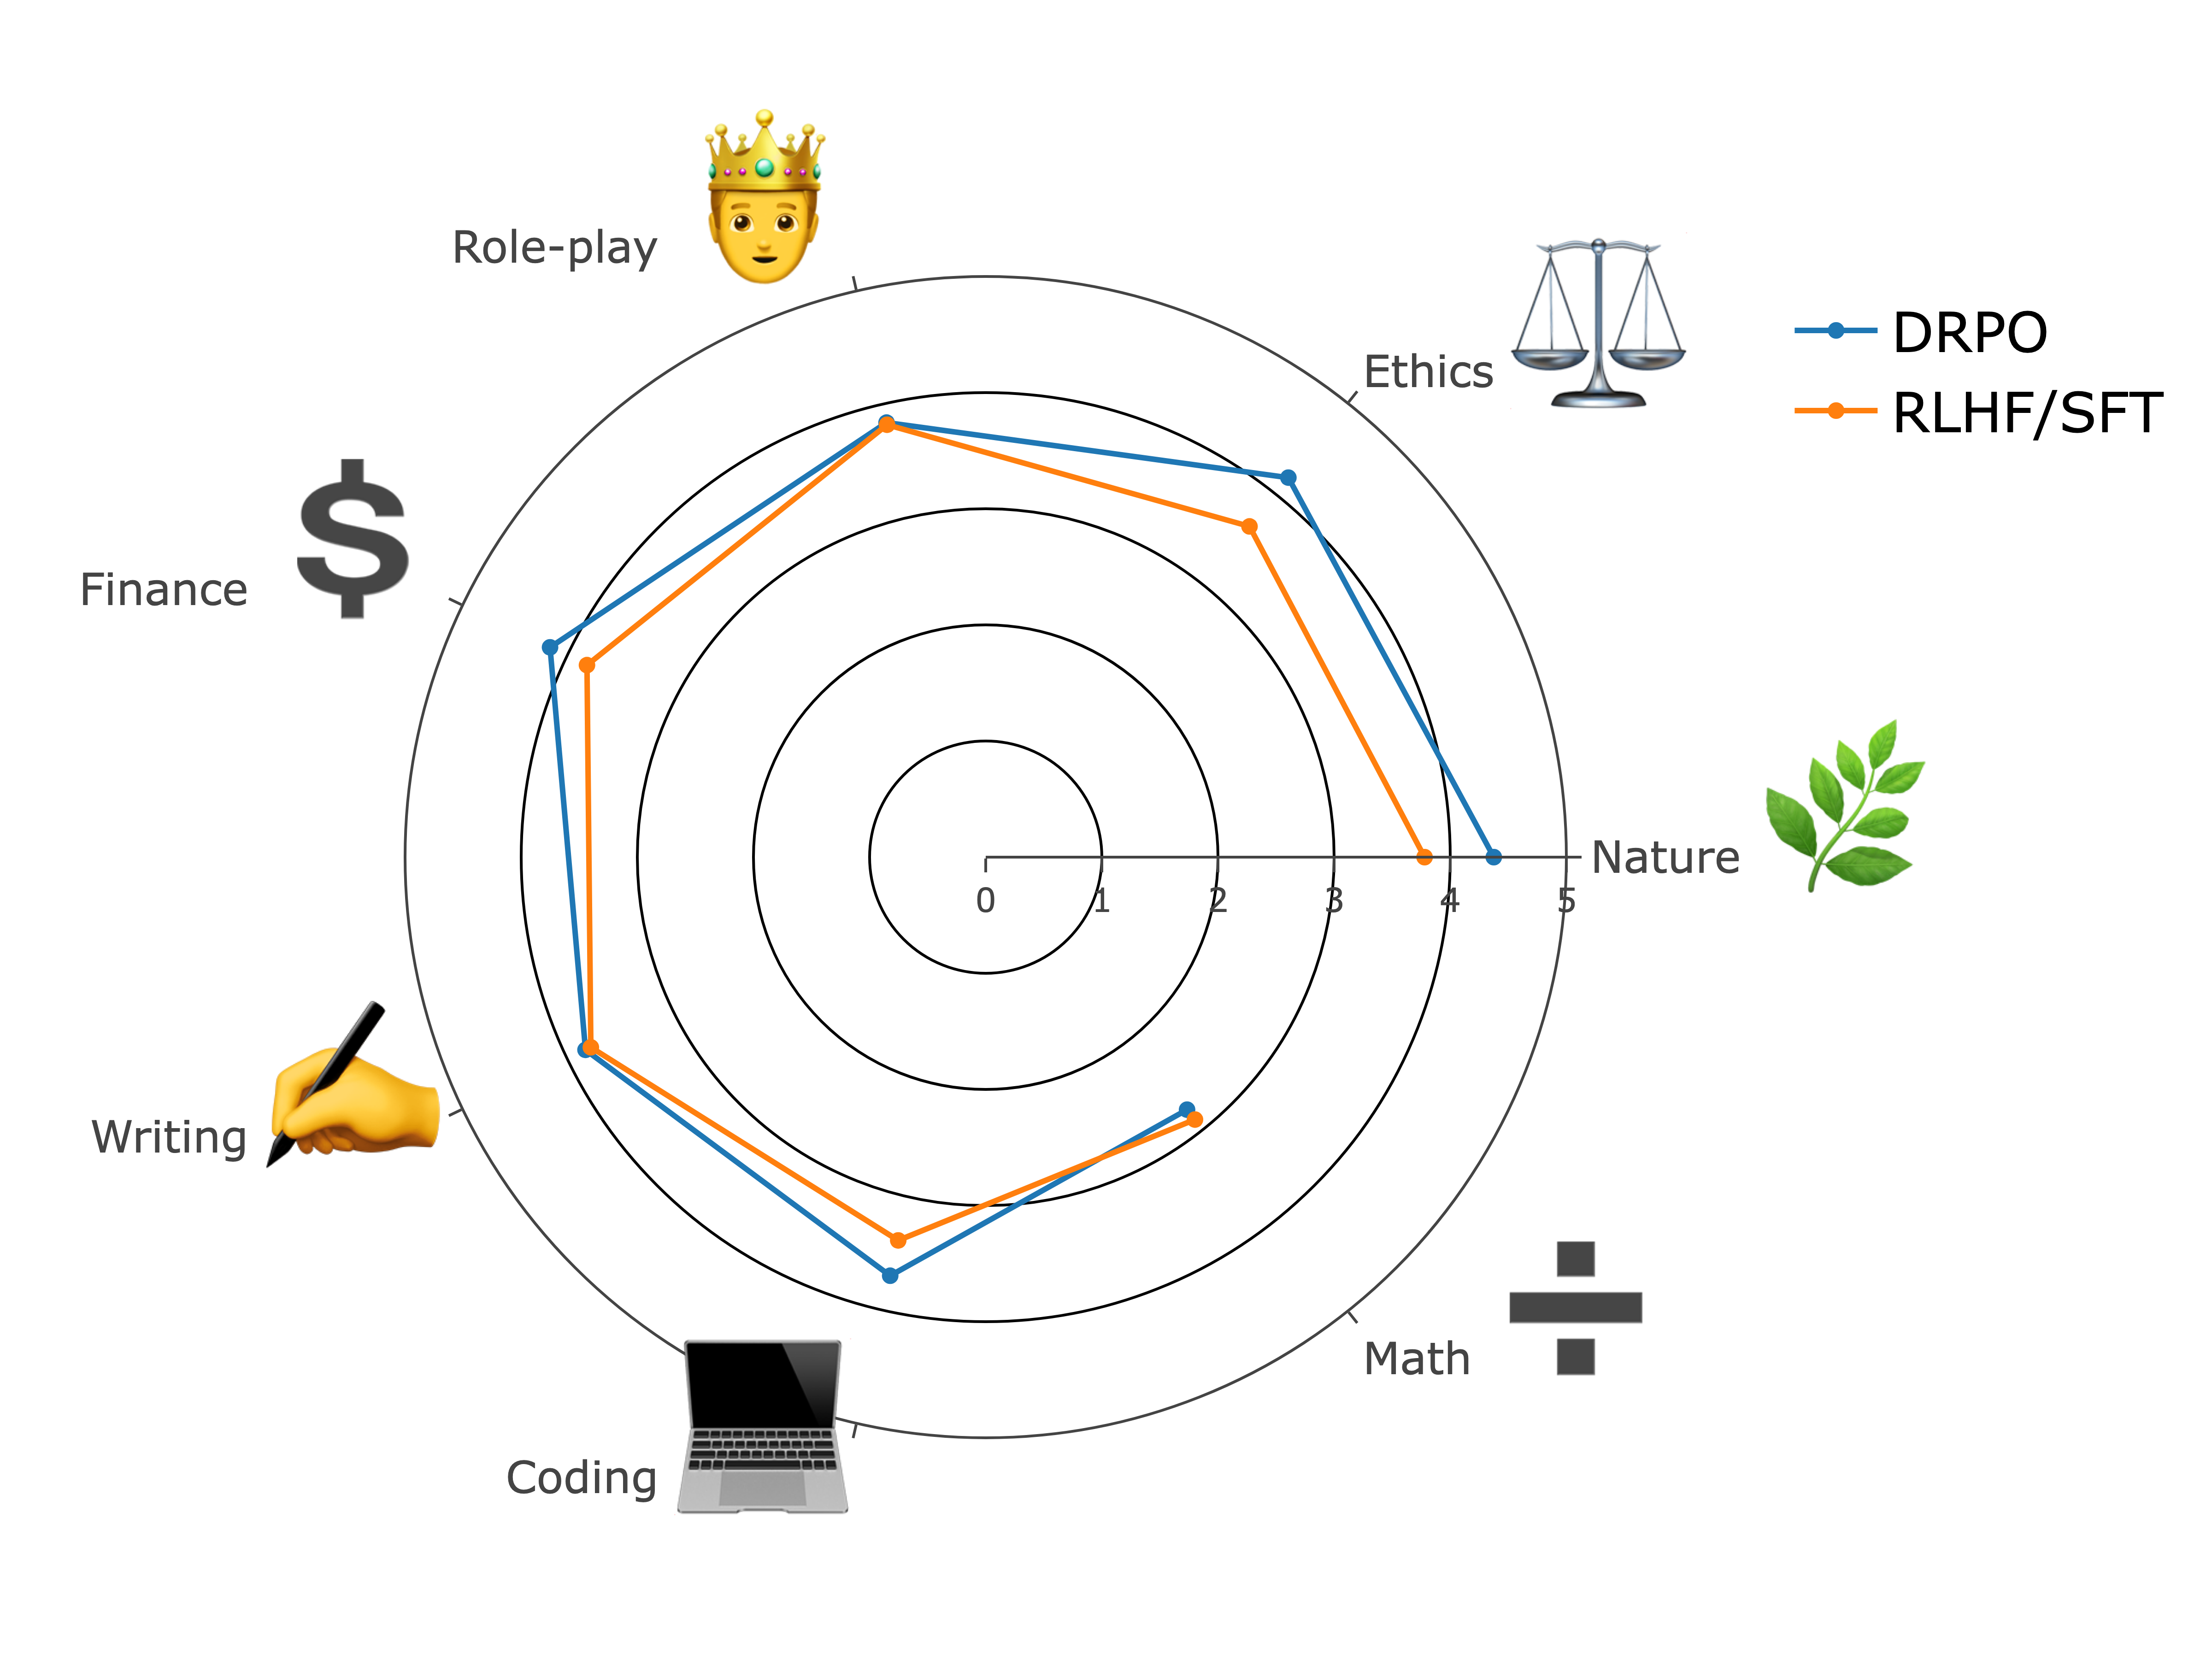
\includegraphics[width=0.95\linewidth]{images/mistral_2.png}
  \label{fig:cat_mistral_2}
\end{subfigure}
\caption{Mistral 7b在各个领域的分类表现。使用\ours,我们可以看到在所有领域的表现都有显著提升。特别是,人文学科、推理、STEM等领域表现出了显著的提升。这凸显了基础模型可以从\ours中获益颇多的事实。}
\label{fig:categorized_performance_mistral}
\end{figure}

\newpage
\subsection{Llama 2 70b}
\begin{figure}[h]
\centering
\begin{subfigure}[b]{.5\textwidth}
  \centering
  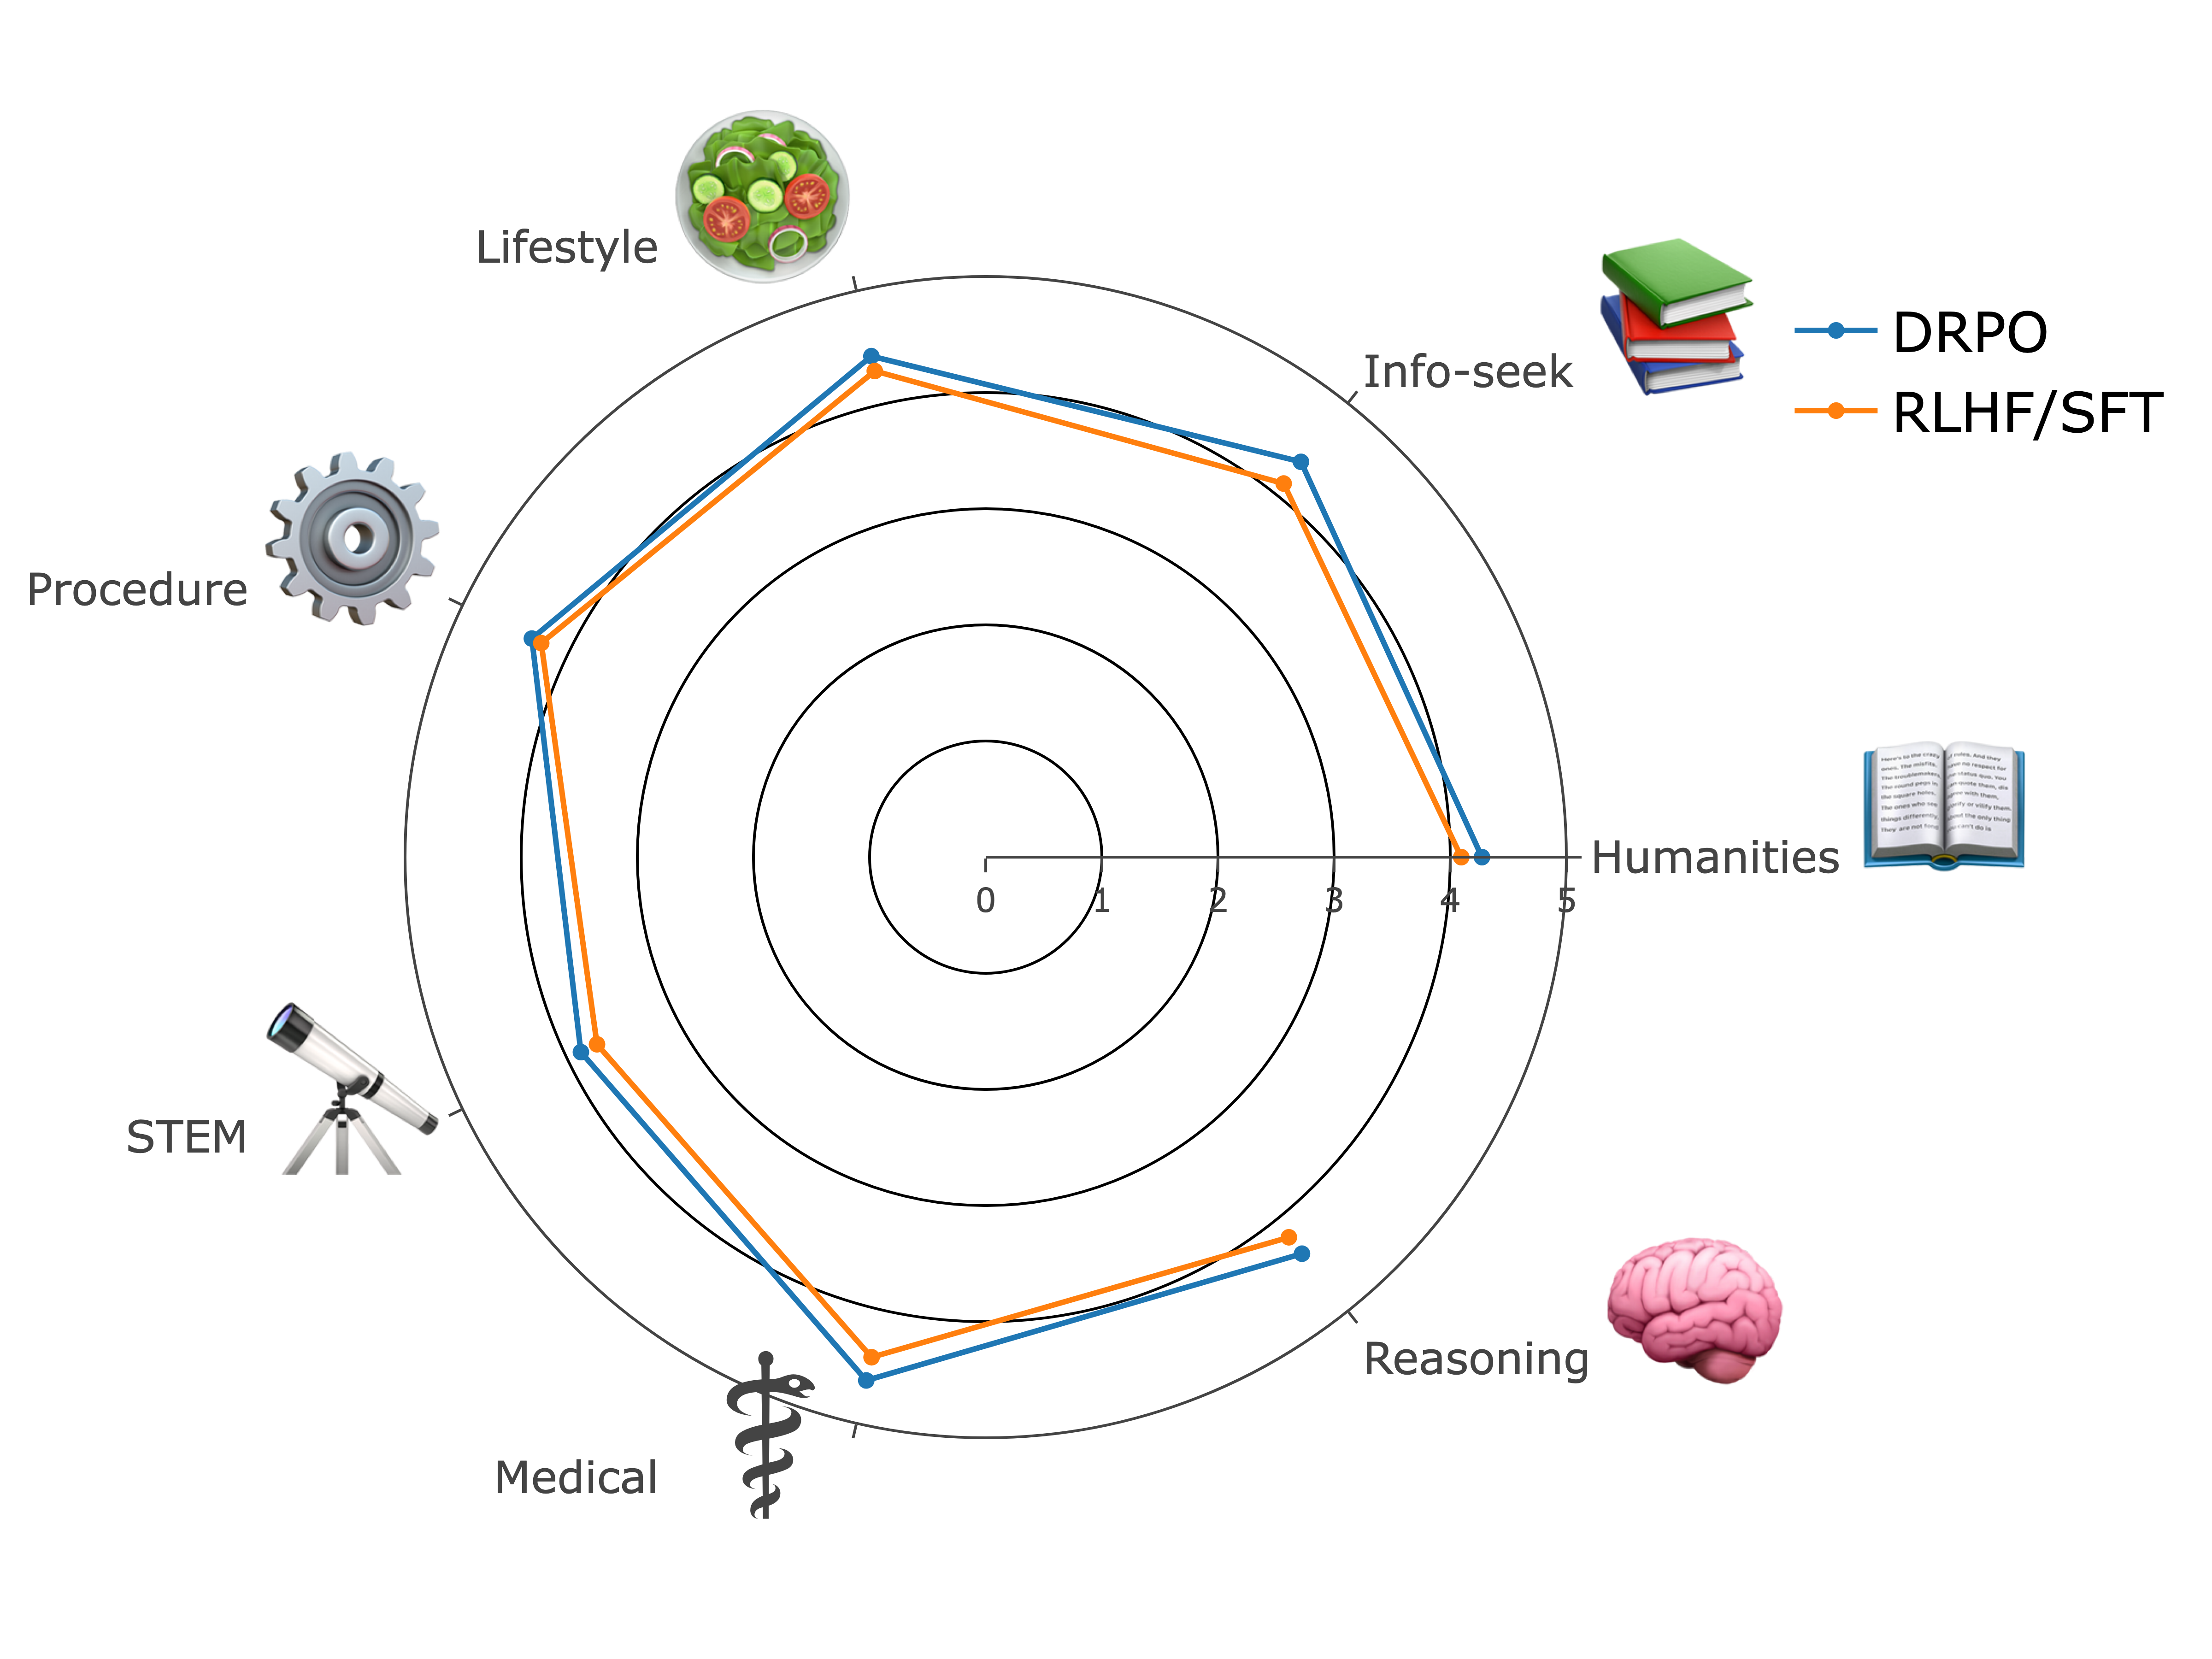
\includegraphics[width=0.95\linewidth]{images/llama_1.png}
  \label{fig:cat_llama_1}
\end{subfigure}

\vspace{1em}

\begin{subfigure}[b]{.5\textwidth}
  \centering
  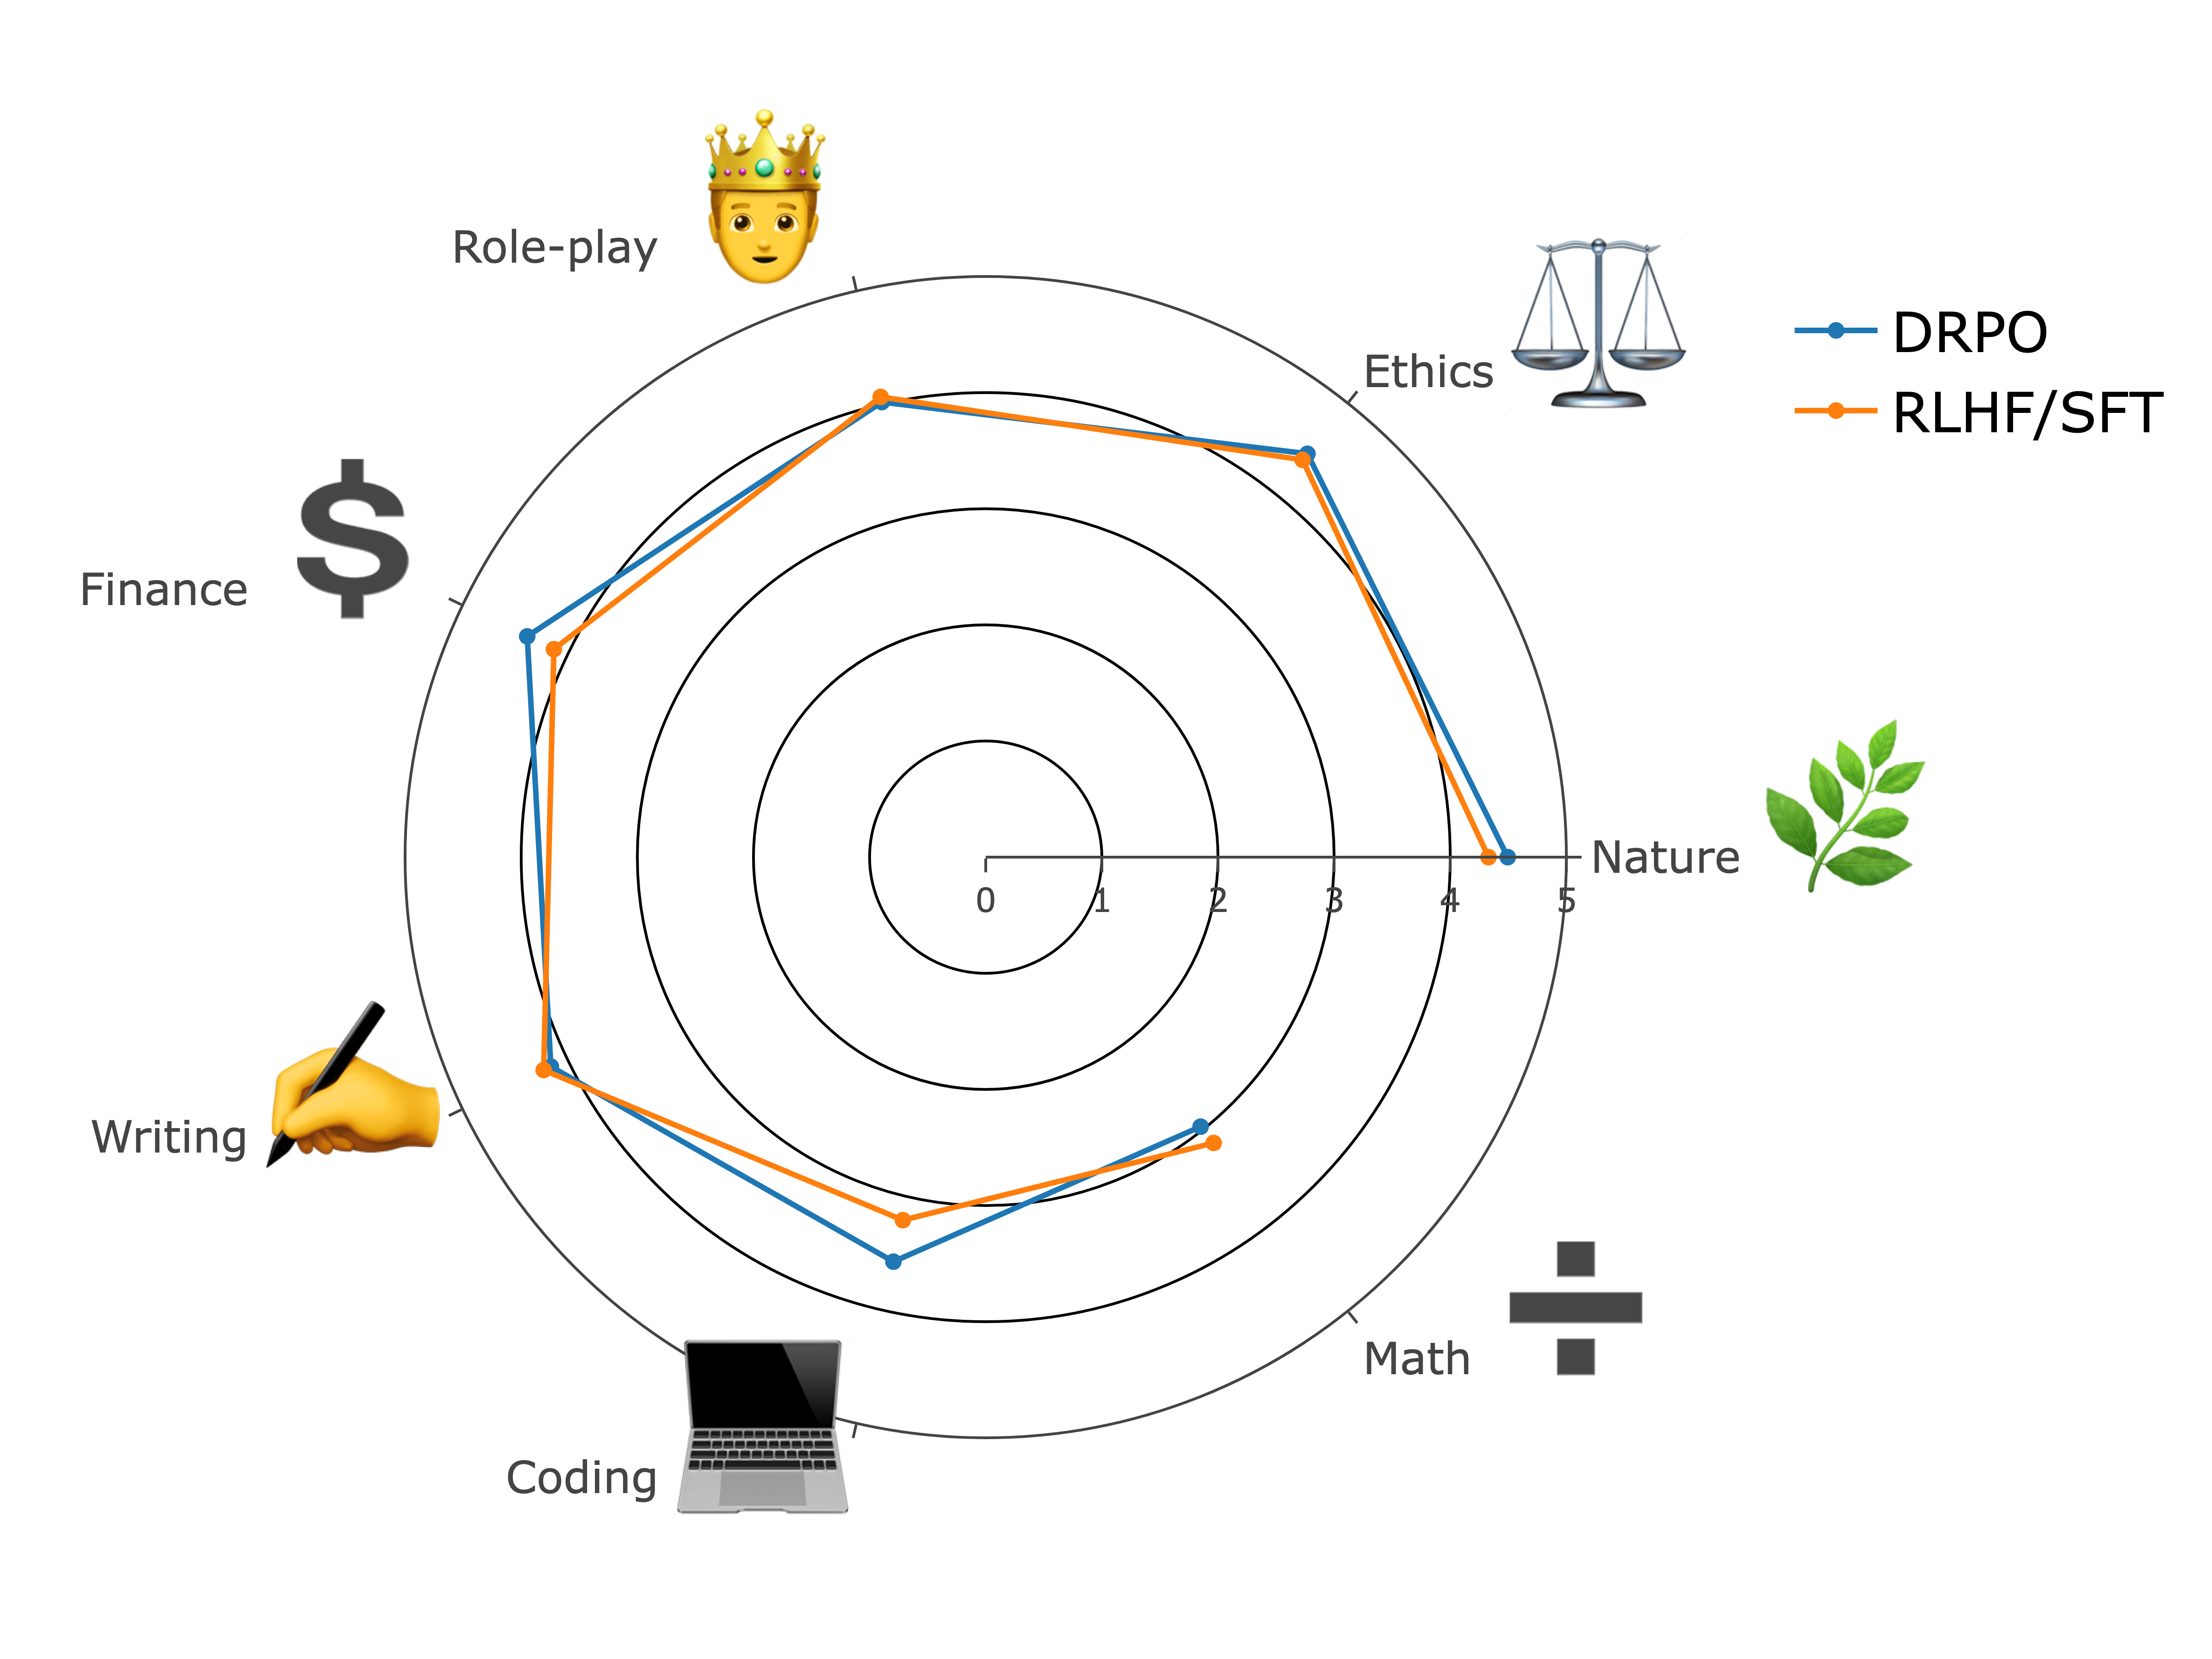
\includegraphics[width=0.95\linewidth]{images/llama_2.png}
  \label{fig:cat_llama_2}
\end{subfigure}
\caption{Llama 2 70$b^q$ 在各个领域的分类性能表现。使用 \ours 后,我们观察到除数学外的所有领域性能均有所提升,而数学领域略有下降。使用 \ours 显著提升了诸如信息检索、编程和金融等领域的性能。}
\label{fig:categorized_performance_llama}
\end{figure}

\newpage
\subsection{\texttt{gpt-3.5-turbo}}

\begin{figure}[h]
\centering
\begin{subfigure}[b]{.5\textwidth}
  \centering
  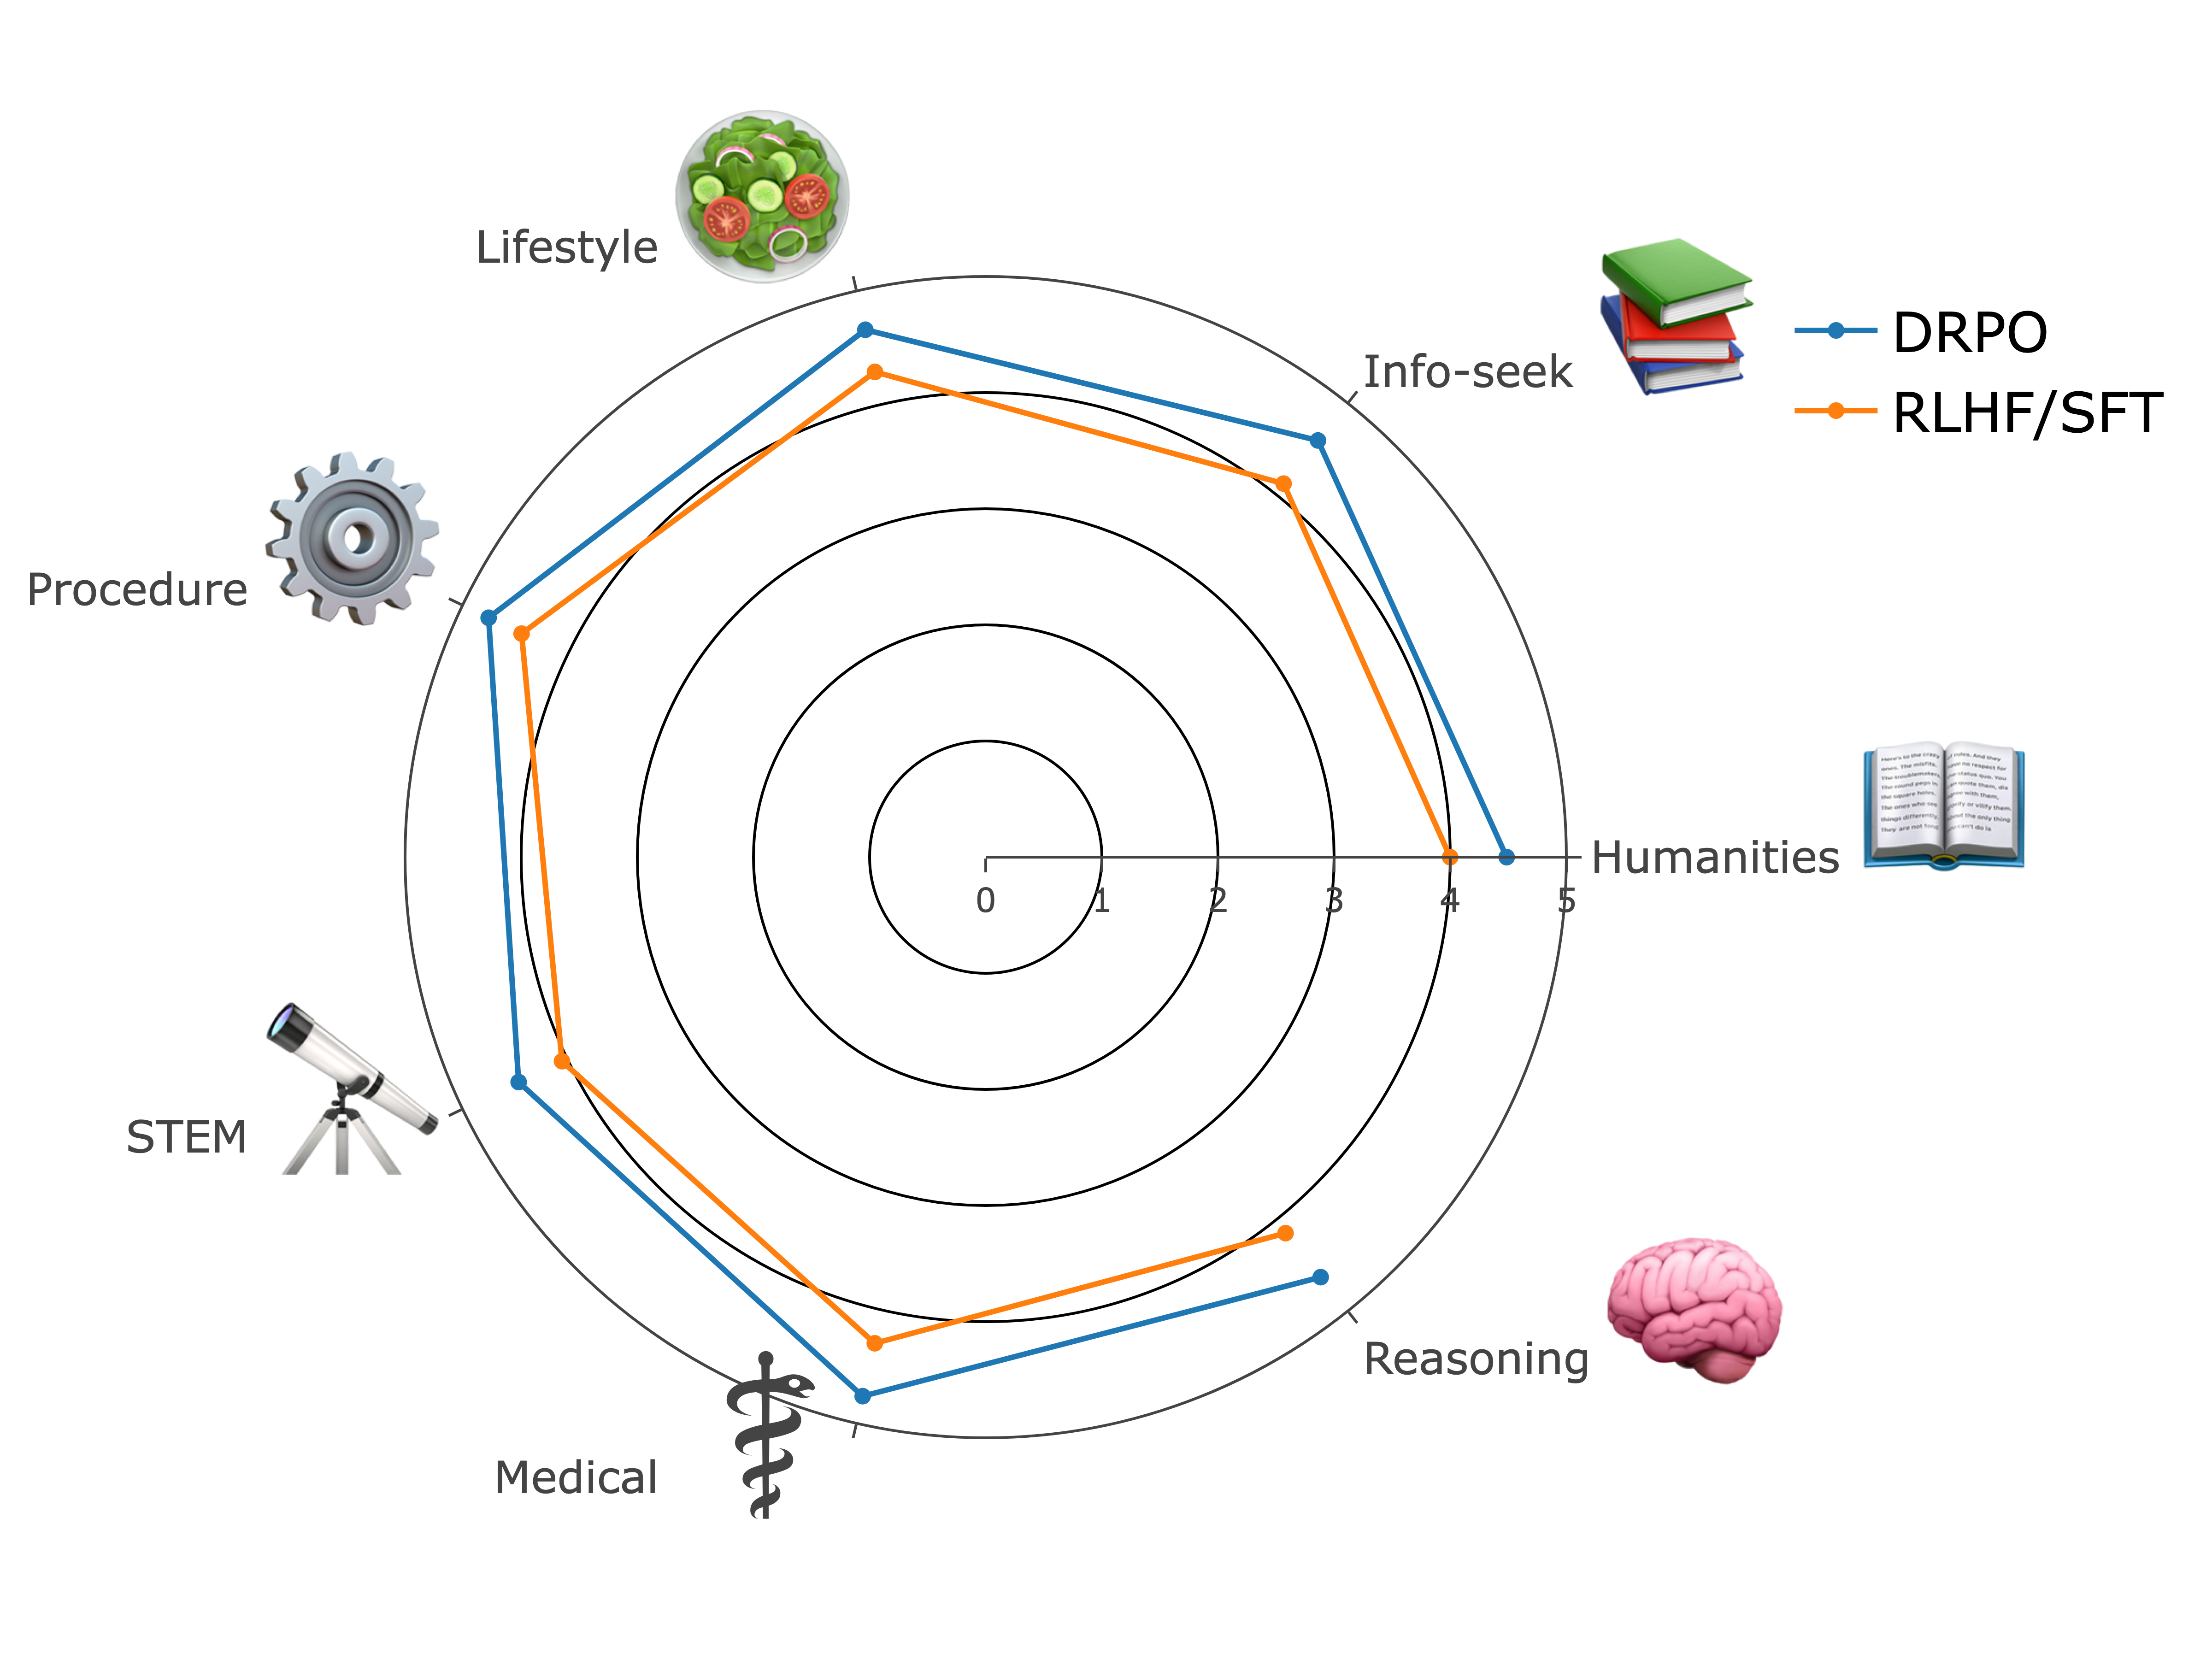
\includegraphics[width=0.95\linewidth]{images/gpt_1.png}
  \label{fig:cat_gpt_1}
\end{subfigure}

\vspace{1em}

\begin{subfigure}[b]{.5\textwidth}
  \centering
  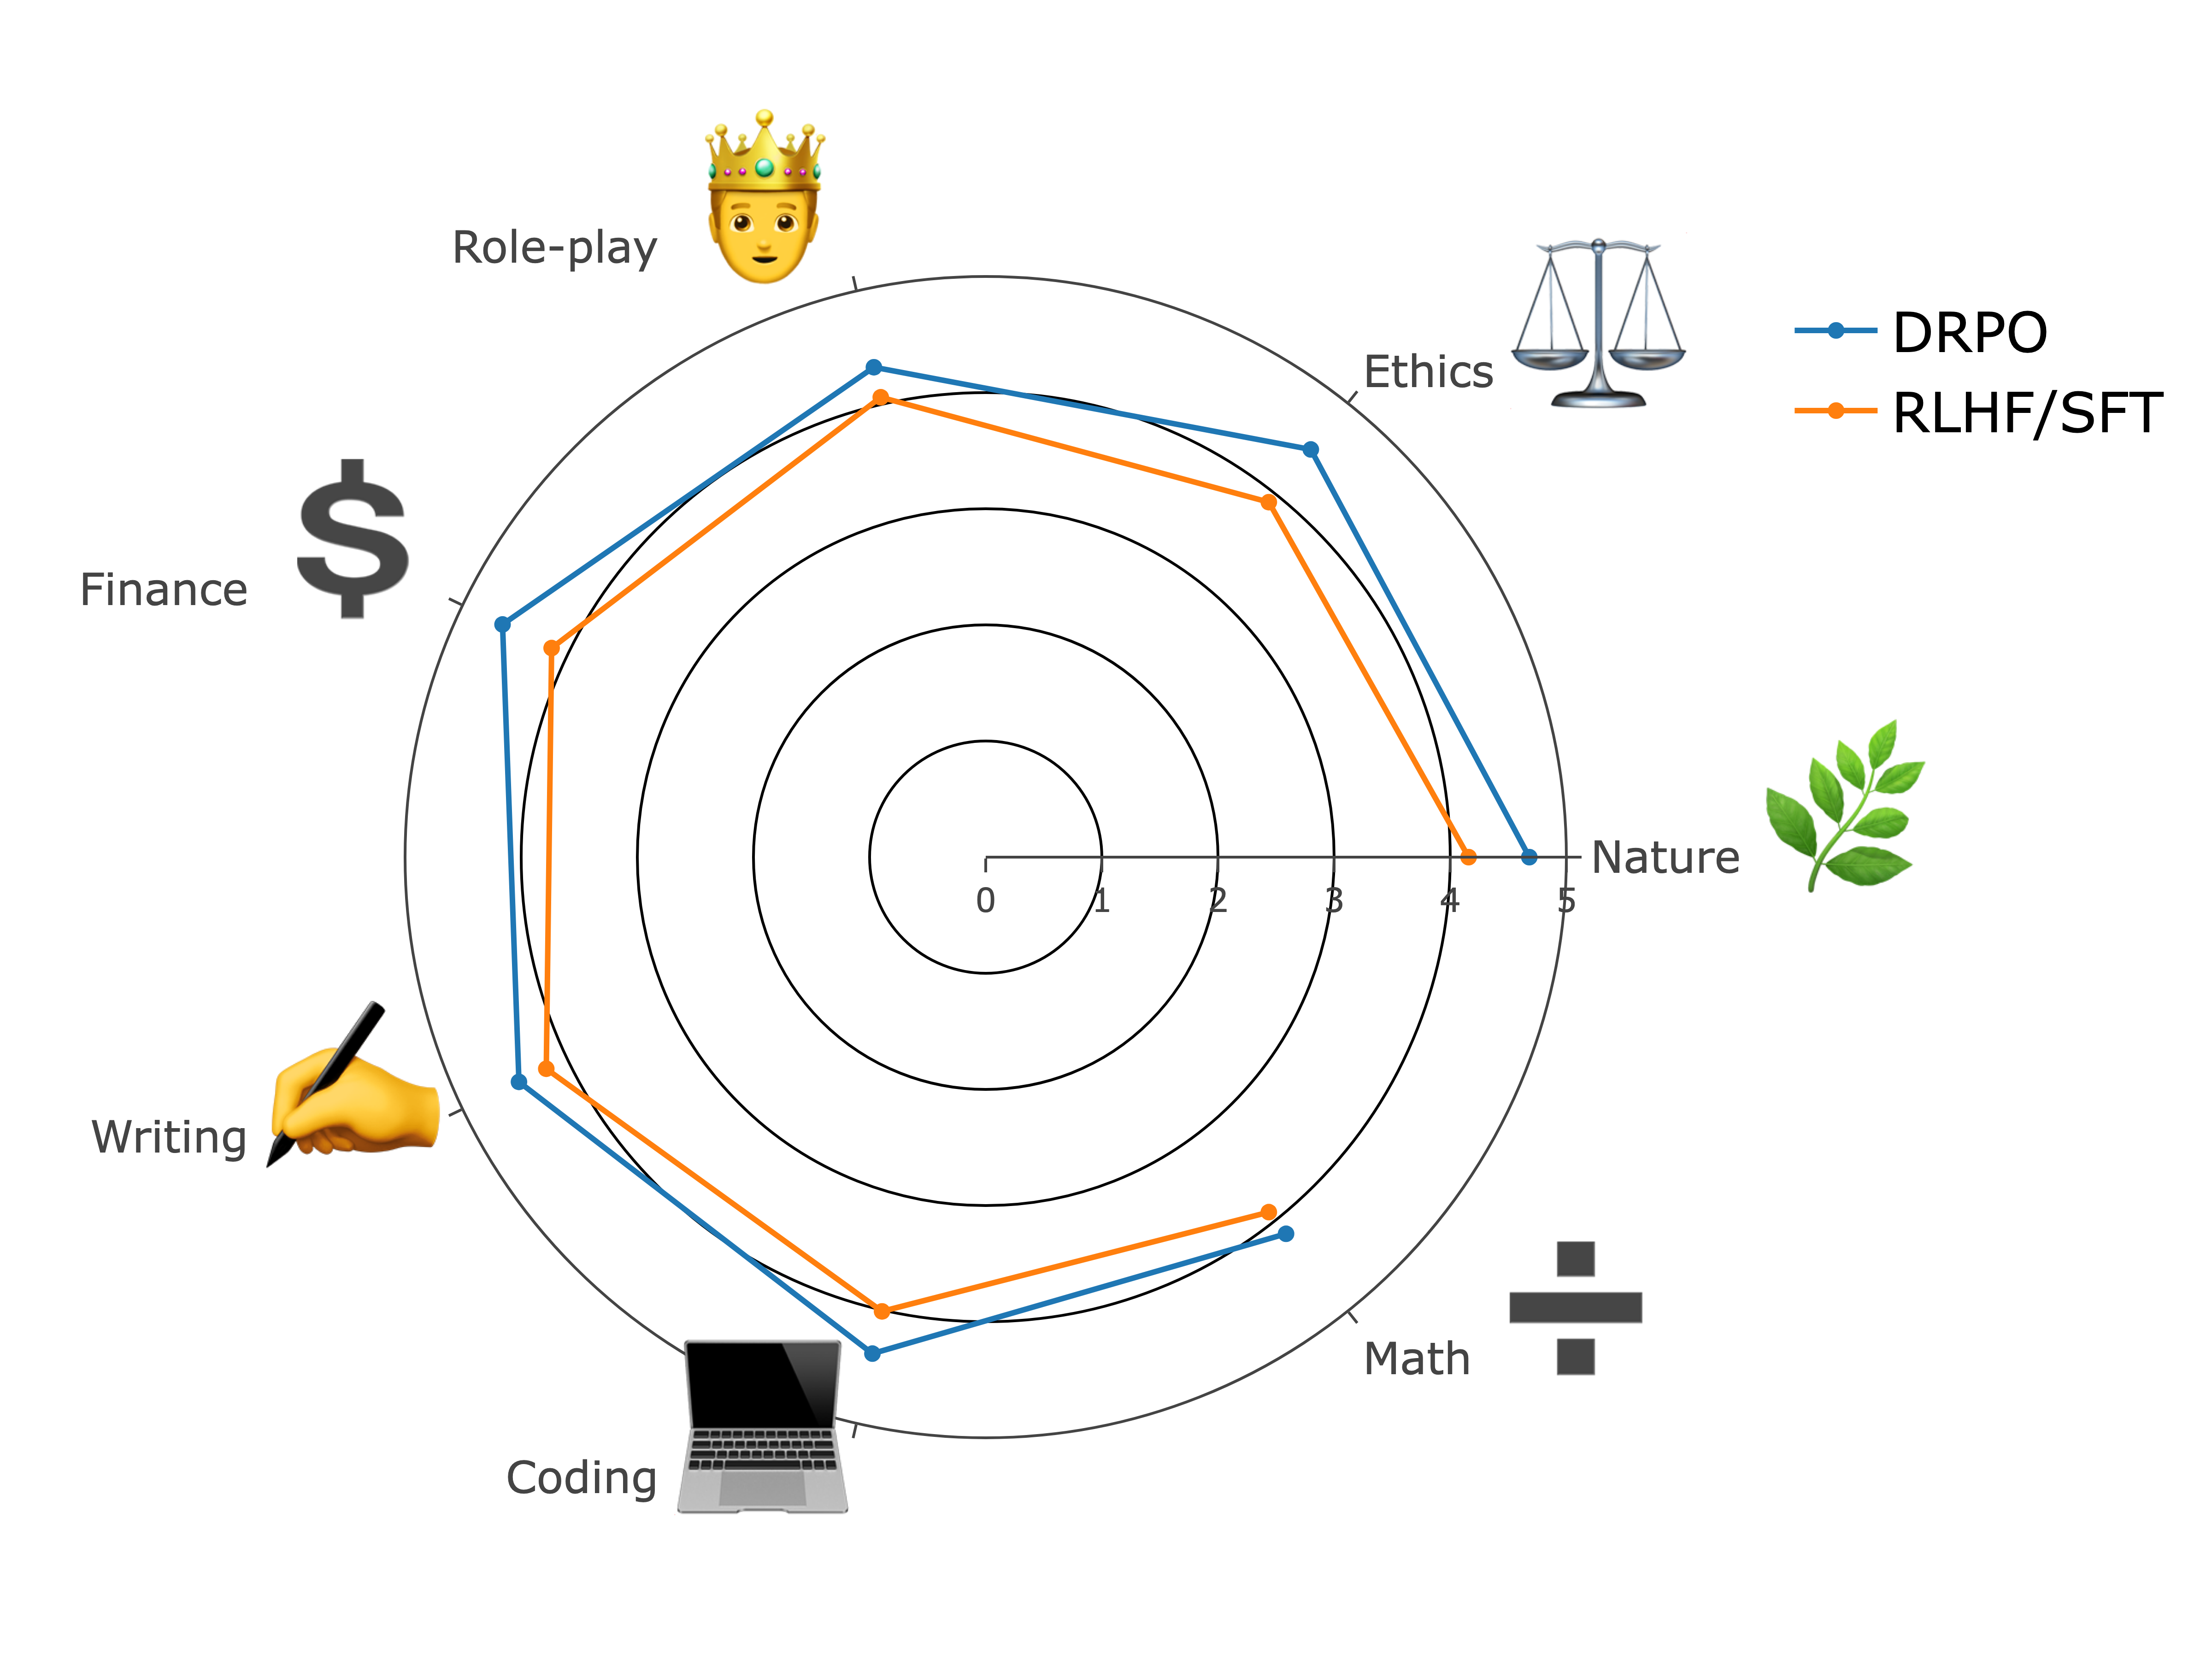
\includegraphics[width=0.95\linewidth]{images/gpt_2.png}
  \label{fig:cat_gpt_2}
\end{subfigure}
\caption{\texttt{gpt-3.5-turbo} 在不同领域的分类性能表现。由于使用了 \ours,该模型在所有领域的性能均有所提升,显示出令人满意的结果。\\
注意:我们将 \ours 方法应用于 RLHF 微调的 \texttt{gpt-3.5-turbo},因为我们无法获取其基础模型。
}
\label{fig:categorized_performance_gpt}
\end{figure}

\newpage

\section{优化算法}
\label{sec:opti_algo}
\subsection{ICL 优化}

\begin{algorithm}[h]
\caption{ICL 优化}\label{alg:icl_opti}

\KwIn{$\mathcal{I}_{base}$,$N$,$\mathcal{O}$,$\mathcal{E}$,$\mathcal{R}$,$D$,$W$,$M$,$\mathcal{T}$}
\KwOut{$\mathcal{I}^{*}$}

\SetKwBlock{Definitions}{定义}{}
\Definitions{

    $\mathcal{I}_{base}$:基础 ICL 示例\;
    $N$:ICL 示例数量\;
    $\mathcal{O}$:优化器\;
    $\mathcal{E}$:评估器\;
    $\mathcal{R}$:奖励函数\;
    $D$:束搜索深度\;
    $W$:束宽度\;
    $M$:每个状态的动作采样次数\;

    $\mathcal{T}: \mathcal{S} \times \mathcal{A} \rightarrow \mathcal{S}$:状态转移函数

}

\For{i $= 1$ 到 $N$}
{
        $(q_i, b_i)$ $ = \mathcal{I}_{\text{base}}[i]$\;
        $s_0 = b_i$ \tcp*[r]{初始化状态}
        使用 $s_0$ 初始化束\;
        \For{t $= 1$ 到 $D$}
        {
            next\_beam = []\;
            \For{j $= 1$ 到 min(len(beam), $W$)}
            {
                $s_{{t-1}_{j}}$ = beam[j]\;
                $r_{{t-1}_j} = \mathcal{R}(s_{{t-1}_{j}} \mid \mathbb{R}_{q_i})$\;

                \SetKwBlock{SampleMtimes}{重复采样 $M$ 次:}{结束}
                \SampleMtimes{
                    $a_{{t-1}_j} = \mathcal{E}(s_{{t-1}_j} \mid \mathbb{R}_{q_i})$\;
                    $s_{t_j} = \mathcal{T}(s_{{t-1}_j}, a_{{t-1}_j})$\;
                    将 $s_{t_j}$ 添加到 \textit{next\_beam}\;
                }
            }
            beam = 从 next\_beam 中选取前 $W$ 个状态\;
        }
        $s^{*}_{\mathcal{D}}$ = 最终束中的最优状态\;
        $\mathcal{I}^*[i] = (q_i, s^{*}_{\mathcal{D}})$\;
}

\Return $\mathcal{I}^*$
\end{algorithm}

\newpage
\subsection{系统提示优化}
\begin{algorithm}[h]
\caption{系统提示优化}\label{alg:prompt_opti}

\KwIn{$\mathcal{I}^*$, $\mathcal{B}$, $\mathcal{O}$, $\mathcal{E}$, $\mathcal{R}$,
$\mathcal{X}$.
$\mathcal{P}$, $D$, $W$, $M$, $\mathcal{T}$}
\KwOut{$\mathcal{P}^{*}$}

\SetKwBlock{Definitions}{定义}{}
\Definitions{

    $\mathcal{I}^*$: 优化后的ICL示例\;
    $\mathcal{B}$: 基础LLM\;
    $\mathcal{O}$: 优化器模型\;
    $\mathcal{E}$: 评估模型\;
    $\mathcal{R}$: 奖励函数\;
    $\mathcal{X}$: 种子数据集\;
    $\mathcal{P}$: 初始系统提示\;
    $D$: 光束深度\;
    $W$: 光束宽度\;
    $M$: 每个状态的动作样本数\;

    $\mathcal{T}: \mathcal{S} \times \mathcal{A} \rightarrow \mathcal{S}$: 转换函数

}

$s_0 = \mathcal{P}$ \tcp*[r]{初始化状态}
初始化光束为 $s_0$\;
\For{t $= 1$ 到 $D$}
{
    $x_{t-1} = \mathcal{X}$[$t-1$]\;
    $\mathcal{I}_K^*$ = 从 $\mathcal{I}^*$ 中选择与 $x_{t-1}$ 最相似的 $K$ 个示例\;
    next\_beam = []\;
    \For{j $= 1$ 到 min(光束长度, $W$)}
    {
        $s_{{t-1}_{j}}$ = 光束[j]\;
        $r_{{t-1}_j} = \mathcal{R}(\mathcal{B}(x_{t-1} \mid s_{{t-1}_{j}}, \mathcal{I}_K^*) \mid \mathbb{R}_{x_{t-1}})$\;

        \SetKwBlock{SampleMtimes}{重复(采样)$M$次:}{结束}
        \SampleMtimes{
            $a_{{t-1}_j} = \mathcal{E}(\mathcal{B}(x_{t-1} \mid s_{{t-1}_{j}}, \mathcal{I}_K^*) \mid \mathbb{R}_{x_{t-1}})$\;
            $s_{t_j} = \mathcal{T}(s_{{t-1}_j}, a_{{t-1}_j})$\;
            将 $s_{t_j}$ 添加到 \textit{next\_beam}\;
        }
    }
    光束 = 从 next\_beam 中选择前 $W$ 个状态\;
}
$s^{*}_{\mathcal{D}}$ = 光束中的最终状态\;
$\mathcal{P}^* = s^{*}_{\mathcal{D}}$\;

\Return $\mathcal{P}^*$
\end{algorithm}

\newpage
\section{优化提示案例研究}
\label{sec:prompt_case_study}

\begin{table}[h]

\definecolor{Gray}{gray}{0.90}
\newcolumntype{a}{>{\columncolor{Gray}}c}
\centering
\resizebox{1\linewidth}{!}{
\begin{tabular}{@{}lp{10cm}@{}}
\toprule
\textbf{模型} & \textbf{优化提示} \\
\midrule
Mistral 7b & \ctext[RGB]{255,225,255}{作为一个有帮助且道德的助手,您的任务是提供不仅准确且安全的回应,同时也要深具吸引力、富有同理心和内容丰富。您的角色是全面理解每个查询的背景,提供展现对主题深刻理解的见解} \ctext[RGB]{255,230,200}{同时兼顾道德考量。您的回答应当加深用户的理解,促进积极的结果,并在能力范围内培养深厚的联系。} \ctext[RGB]{255,230,230}{至关重要的是直接回应用户的查询,提供简洁而全面的信息,}\ctext[RGB]{233,252,232}{并明确告知您的局限性。}\ctext[RGB]{255,230,230}{通过使您的回答更具吸引力、创造性和人性化,来提升用户体验。}
\ctext[RGB]{233,252,232}{- 您无法访问互联网或实时数据,也不能执行实际操作。避免尝试回答需要此类能力的问题。}
\ctext[RGB]{255,230,200}{- 避免涉及可能促成非法活动、伤害他人或不道德行为的问题。相反,应提供解释或建议合法和积极的替代方案。}
\ctext[RGB]{255,230,230}{- 努力发挥创造力,使用生动的语言,融入讲故事的元素,并提供与用户相关的例子。}
\ctext[RGB]{233,252,232}{- 避免冷冰冰的语气,通过变换句子结构,采用对话风格,并在回答中加入温暖与同理心元素。}
\ctext[RGB]{255,225,255}{- 优先确保清晰简洁,确保您的回答易于所有用户理解,并避免不必要的重复。}
\ctext[RGB]{233,252,232}{- 鼓励批判性思维,通过提出多种观点或考虑因素,邀请用户进一步探索该话题。}
\ctext[RGB]{255,230,200}{- 公开说明某些回答的推测性质及您的局限性,建议进一步探讨的领域或相关话题,可能会提供额外的见解。}
 \\ \midrule
\texttt{gpt-3.5-turbo} & \ctext[RGB]{255,225,255}{作为一个有帮助且道德的助手,您的主要目标是提供准确、吸引人、清晰且情感共鸣的回答,涵盖各种查询。您的回答应深植于事实信息中,同时在适当时也提供深思熟虑的推测和对话题的探索。} \ctext[RGB]{230, 230, 255}{深入探讨作者意图、历史背景和文化意义是至关重要的,这有助于增加深度并激发批判性思维。}\ctext[RGB]{230,246,255}{努力让复杂的主题变得易于理解并富有情感共鸣,以人性化和相关的方式进行沟通。组织您的回答以提升可读性和情感连接,避免过于技术化的行话。} \ctext[RGB]{233,252,232}{面对局限性或请求有害信息时,优先考虑安全性、合法性和道德考量。}
\ctext[RGB]{255,225,255}{始终承认您的知识局限,尤其是在推测历史“假设”情境、未来预测或情感解读时。公开说明您无法访问实时数据或执行实际操作,并建议安全、合法的替代话题。}
\ctext[RGB]{230,246,255}{在详细、信息丰富的内容和对话式、吸引人的语气之间找到平衡。通过讲故事、举例、使用类比和直接提问的方式让信息更具相关性。} \ctext[RGB]{230,246,255}{避免用过多的信息淹没用户;组织您的回答以确保清晰、条理清楚,并考虑到用户的认知负担。}
 \\

 \bottomrule
\end{tabular}
}
\label{tab:opti_prompt_case_study}
\caption{
\ours为Mistral 7b和\texttt{gpt-3.5-turbo}优化提示的对比。\ours自定义提示以识别并修复特定模型的对齐问题。(颜色标签的语义见下文。)
}
\end{table}


我们通过颜色突出显示了优化提示的不同方面,包括\ctext[RGB]{233,252,232}{如无法访问实时数据的局限性},\ctext[RGB]{255,230,230}{针对小模型如Mistral 7b的避免重复的指导},\ctext[RGB]{230,246,255}{针对大模型如\texttt{gpt-3.5-turbo}的避免行话的指导},\ctext[RGB]{255,230,200}{道德指导},\ctext[RGB]{255,225,255}{AI助手的通用指导},\ctext[RGB]{230, 230, 255}{提高回答参与度的提示}。

\newpage

\section{元提示}
\label{sec:meta_prompts}
\subsection{奖励提示}

在本节中,我们介绍了用于计算总体奖励的提示。奖励提示使用了像 eval$\_$dict 和奖励选择提示等组件。我们首先使用奖励选择提示(如节 \ref{sec:reward_selection_prompt} 中所示)来选择适当的奖励,然后为所选奖励创建一个格式如节 \ref{sec:eval_dict} 中所示的 eval$\_$dict。最后,使用奖励列表和 eval$\_$dict,我们使用如下所示的奖励提示来计算动态奖励。

\begin{lstlisting}[breaklines=true,breakatwhitespace=true]

Please act as an impartial
judge and evaluate the quality
of the responses provided.
You will rate the quality
of the output based on
several selected aspects.

## Query:
[QUERY]

## Output:
[OUTPUT]

## Evaluate
### Aspects

Below is a list of
aspects for evaluating
the quality of the response:
[ASPECT_LIST]

These aspects are selected
for the following reasons:
[ASPECT_REASON]

### Format

Given the query, please rate the quality of the output by scoring it from 1 to 5 individually on **each aspect**.
- 1: strongly disagree
- 2: disagree
- 3: neutral
- 4: agree
- 5: strongly agree

Now, please output your scores and a short rationale below in a JSON format by filling in the placeholders in []:
```
[EVAL_DICT]
```
\end{lstlisting}
\subsubsection{评估字典}  
\label{sec:eval_dict}  
\begin{lstlisting}[breaklines=true,breakatwhitespace=true]

{"Helpfulness": {
        "rationale": "[your thoughts on the helpfulness of the response]",
        "score": "[your helpfulness score]"
    },
    "Clarity": {
        "rationale": "[your thoughts on the clarity of the response]",
        "score": "[your clarity score]"
    },
    "Factuality": {
        "rationale": "[your thoughts on the factuality of the response]",
        "score": "[your factuality score]"
    },
    "Depth": {
        "rationale": "[your thoughts on the depth of the response]",
        "score": "[your depth score]"
    },
    ...... for all chosen rewards
}

\end{lstlisting}  \subsubsection{评估字典}  
\label{sec:eval_dict}  
\begin{lstlisting}[breaklines=true,breakatwhitespace=true]

{"Helpfulness": {
        "rationale": "[your thoughts on the helpfulness of the response]",
        "score": "[your helpfulness score]"
    },
    "Clarity": {
        "rationale": "[your thoughts on the clarity of the response]",
        "score": "[your clarity score]"
    },
    "Factuality": {
        "rationale": "[your thoughts on the factuality of the response]",
        "score": "[your factuality score]"
    },
    "Depth": {
        "rationale": "[your thoughts on the depth of the response]",
        "score": "[your depth score]"
    },
    ...... for all chosen rewards
}

\end{lstlisting}  \subsubsection{评估字典}  
\label{sec:eval_dict}  
\begin{lstlisting}[breaklines=true,breakatwhitespace=true]

{"Helpfulness": {
        "rationale": "[your thoughts on the helpfulness of the response]",
        "score": "[your helpfulness score]"
    },
    "Clarity": {
        "rationale": "[your thoughts on the clarity of the response]",
        "score": "[your clarity score]"
    },
    "Factuality": {
        "rationale": "[your thoughts on the factuality of the response]",
        "score": "[your factuality score]"
    },
    "Depth": {
        "rationale": "[your thoughts on the depth of the response]",
        "score": "[your depth score]"
    },
    ...... for all chosen rewards
}

\end{lstlisting}  \subsubsection{评估字典}  
\label{sec:eval_dict}  
\begin{lstlisting}[breaklines=true,breakatwhitespace=true]

{"Helpfulness": {
        "rationale": "[your thoughts on the helpfulness of the response]",
        "score": "[your helpfulness score]"
    },
    "Clarity": {
        "rationale": "[your thoughts on the clarity of the response]",
        "score": "[your clarity score]"
    },
    "Factuality": {
        "rationale": "[your thoughts on the factuality of the response]",
        "score": "[your factuality score]"
    },
    "Depth": {
        "rationale": "[your thoughts on the depth of the response]",
        "score": "[your depth score]"
    },
    ...... for all chosen rewards
}

\end{lstlisting}  \subsubsection{评估字典}  
\label{sec:eval_dict}  
\begin{lstlisting}[breaklines=true,breakatwhitespace=true]

{"Helpfulness": {
        "rationale": "[your thoughts on the helpfulness of the response]",
        "score": "[your helpfulness score]"
    },
    "Clarity": {
        "rationale": "[your thoughts on the clarity of the response]",
        "score": "[your clarity score]"
    },
    "Factuality": {
        "rationale": "[your thoughts on the factuality of the response]",
        "score": "[your factuality score]"
    },
    "Depth": {
        "rationale": "[your thoughts on the depth of the response]",
        "score": "[your depth score]"
    },
    ...... for all chosen rewards
}

\end{lstlisting}  \subsubsection{评估字典}  
\label{sec:eval_dict}  
\begin{lstlisting}[breaklines=true,breakatwhitespace=true]

{"Helpfulness": {
        "rationale": "[your thoughts on the helpfulness of the response]",
        "score": "[your helpfulness score]"
    },
    "Clarity": {
        "rationale": "[your thoughts on the clarity of the response]",
        "score": "[your clarity score]"
    },
    "Factuality": {
        "rationale": "[your thoughts on the factuality of the response]",
        "score": "[your factuality score]"
    },
    "Depth": {
        "rationale": "[your thoughts on the depth of the response]",
        "score": "[your depth score]"
    },
    ...... for all chosen rewards
}

\end{lstlisting}  \subsubsection{评估字典}  
\label{sec:eval_dict}  
\begin{lstlisting}[breaklines=true,breakatwhitespace=true]

{"Helpfulness": {
        "rationale": "[your thoughts on the helpfulness of the response]",
        "score": "[your helpfulness score]"
    },
    "Clarity": {
        "rationale": "[your thoughts on the clarity of the response]",
        "score": "[your clarity score]"
    },
    "Factuality": {
        "rationale": "[your thoughts on the factuality of the response]",
        "score": "[your factuality score]"
    },
    "Depth": {
        "rationale": "[your thoughts on the depth of the response]",
        "score": "[your depth score]"
    },
    ...... for all chosen rewards
}

\end{lstlisting}  \subsubsection{评估字典}  
\label{sec:eval_dict}  
\begin{lstlisting}[breaklines=true,breakatwhitespace=true]

{"Helpfulness": {
        "rationale": "[your thoughts on the helpfulness of the response]",
        "score": "[your helpfulness score]"
    },
    "Clarity": {
        "rationale": "[your thoughts on the clarity of the response]",
        "score": "[your clarity score]"
    },
    "Factuality": {
        "rationale": "[your thoughts on the factuality of the response]",
        "score": "[your factuality score]"
    },
    "Depth": {
        "rationale": "[your thoughts on the depth of the response]",
        "score": "[your depth score]"
    },
    ...... for all chosen rewards
}

\end{lstlisting}  \subsubsection{评估字典}  
\label{sec:eval_dict}  
\begin{lstlisting}[breaklines=true,breakatwhitespace=true]

{"Helpfulness": {
        "rationale": "[your thoughts on the helpfulness of the response]",
        "score": "[your helpfulness score]"
    },
    "Clarity": {
        "rationale": "[your thoughts on the clarity of the response]",
        "score": "[your clarity score]"
    },
    "Factuality": {
        "rationale": "[your thoughts on the factuality of the response]",
        "score": "[your factuality score]"
    },
    "Depth": {
        "rationale": "[your thoughts on the depth of the response]",
        "score": "[your depth score]"
    },
    ...... for all chosen rewards
}

\end{lstlisting}  \subsubsection{评估字典}  
\label{sec:eval_dict}  
\begin{lstlisting}[breaklines=true,breakatwhitespace=true]

{"Helpfulness": {
        "rationale": "[your thoughts on the helpfulness of the response]",
        "score": "[your helpfulness score]"
    },
    "Clarity": {
        "rationale": "[your thoughts on the clarity of the response]",
        "score": "[your clarity score]"
    },
    "Factuality": {
        "rationale": "[your thoughts on the factuality of the response]",
        "score": "[your factuality score]"
    },
    "Depth": {
        "rationale": "[your thoughts on the depth of the response]",
        "score": "[your depth score]"
    },
    ...... for all chosen rewards
}

\end{lstlisting}  \subsubsection{评估字典}  
\label{sec:eval_dict}  
\begin{lstlisting}[breaklines=true,breakatwhitespace=true]

{"Helpfulness": {
        "rationale": "[your thoughts on the helpfulness of the response]",
        "score": "[your helpfulness score]"
    },
    "Clarity": {
        "rationale": "[your thoughts on the clarity of the response]",
        "score": "[your clarity score]"
    },
    "Factuality": {
        "rationale": "[your thoughts on the factuality of the response]",
        "score": "[your factuality score]"
    },
    "Depth": {
        "rationale": "[your thoughts on the depth of the response]",
        "score": "[your depth score]"
    },
    ...... for all chosen rewards
}

\end{lstlisting}  \subsubsection{评估字典}  
\label{sec:eval_dict}  
\begin{lstlisting}[breaklines=true,breakatwhitespace=true]

{"Helpfulness": {
        "rationale": "[your thoughts on the helpfulness of the response]",
        "score": "[your helpfulness score]"
    },
    "Clarity": {
        "rationale": "[your thoughts on the clarity of the response]",
        "score": "[your clarity score]"
    },
    "Factuality": {
        "rationale": "[your thoughts on the factuality of the response]",
        "score": "[your factuality score]"
    },
    "Depth": {
        "rationale": "[your thoughts on the depth of the response]",
        "score": "[your depth score]"
    },
    ...... for all chosen rewards
}

\end{lstlisting}  \subsubsection{评估字典}  
\label{sec:eval_dict}  
\begin{lstlisting}[breaklines=true,breakatwhitespace=true]

{"Helpfulness": {
        "rationale": "[your thoughts on the helpfulness of the response]",
        "score": "[your helpfulness score]"
    },
    "Clarity": {
        "rationale": "[your thoughts on the clarity of the response]",
        "score": "[your clarity score]"
    },
    "Factuality": {
        "rationale": "[your thoughts on the factuality of the response]",
        "score": "[your factuality score]"
    },
    "Depth": {
        "rationale": "[your thoughts on the depth of the response]",
        "score": "[your depth score]"
    },
    ...... for all chosen rewards
}

\end{lstlisting}  \subsubsection{评估字典}  
\label{sec:eval_dict}  
\begin{lstlisting}[breaklines=true,breakatwhitespace=true]

{"Helpfulness": {
        "rationale": "[your thoughts on the helpfulness of the response]",
        "score": "[your helpfulness score]"
    },
    "Clarity": {
        "rationale": "[your thoughts on the clarity of the response]",
        "score": "[your clarity score]"
    },
    "Factuality": {
        "rationale": "[your thoughts on the factuality of the response]",
        "score": "[your factuality score]"
    },
    "Depth": {
        "rationale": "[your thoughts on the depth of the response]",
        "score": "[your depth score]"
    },
    ...... for all chosen rewards
}

\end{lstlisting}  \subsubsection{评估字典}  
\label{sec:eval_dict}  
\begin{lstlisting}[breaklines=true,breakatwhitespace=true]

{"Helpfulness": {
        "rationale": "[your thoughts on the helpfulness of the response]",
        "score": "[your helpfulness score]"
    },
    "Clarity": {
        "rationale": "[your thoughts on the clarity of the response]",
        "score": "[your clarity score]"
    },
    "Factuality": {
        "rationale": "[your thoughts on the factuality of the response]",
        "score": "[your factuality score]"
    },
    "Depth": {
        "rationale": "[your thoughts on the depth of the response]",
        "score": "[your depth score]"
    },
    ...... for all chosen rewards
}

\end{lstlisting}  \subsubsection{评估字典}  
\label{sec:eval_dict}  
\begin{lstlisting}[breaklines=true,breakatwhitespace=true]

{"Helpfulness": {
        "rationale": "[your thoughts on the helpfulness of the response]",
        "score": "[your helpfulness score]"
    },
    "Clarity": {
        "rationale": "[your thoughts on the clarity of the response]",
        "score": "[your clarity score]"
    },
    "Factuality": {
        "rationale": "[your thoughts on the factuality of the response]",
        "score": "[your factuality score]"
    },
    "Depth": {
        "rationale": "[your thoughts on the depth of the response]",
        "score": "[your depth score]"
    },
    ...... for all chosen rewards
}

\end{lstlisting}  \subsubsection{评估字典}  
\label{sec:eval_dict}  
\begin{lstlisting}[breaklines=true,breakatwhitespace=true]

{"Helpfulness": {
        "rationale": "[your thoughts on the helpfulness of the response]",
        "score": "[your helpfulness score]"
    },
    "Clarity": {
        "rationale": "[your thoughts on the clarity of the response]",
        "score": "[your clarity score]"
    },
    "Factuality": {
        "rationale": "[your thoughts on the factuality of the response]",
        "score": "[your factuality score]"
    },
    "Depth": {
        "rationale": "[your thoughts on the depth of the response]",
        "score": "[your depth score]"
    },
    ...... for all chosen rewards
}

\end{lstlisting}  \subsubsection{评估字典}  
\label{sec:eval_dict}  
\begin{lstlisting}[breaklines=true,breakatwhitespace=true]

{"Helpfulness": {
        "rationale": "[your thoughts on the helpfulness of the response]",
        "score": "[your helpfulness score]"
    },
    "Clarity": {
        "rationale": "[your thoughts on the clarity of the response]",
        "score": "[your clarity score]"
    },
    "Factuality": {
        "rationale": "[your thoughts on the factuality of the response]",
        "score": "[your factuality score]"
    },
    "Depth": {
        "rationale": "[your thoughts on the depth of the response]",
        "score": "[your depth score]"
    },
    ...... for all chosen rewards
}

\end{lstlisting}  \subsubsection{评估字典}  
\label{sec:eval_dict}  
\begin{lstlisting}[breaklines=true,breakatwhitespace=true]

{"Helpfulness": {
        "rationale": "[your thoughts on the helpfulness of the response]",
        "score": "[your helpfulness score]"
    },
    "Clarity": {
        "rationale": "[your thoughts on the clarity of the response]",
        "score": "[your clarity score]"
    },
    "Factuality": {
        "rationale": "[your thoughts on the factuality of the response]",
        "score": "[your factuality score]"
    },
    "Depth": {
        "rationale": "[your thoughts on the depth of the response]",
        "score": "[your depth score]"
    },
    ...... for all chosen rewards
}

\end{lstlisting}  \subsubsection{评估字典}  
\label{sec:eval_dict}  
\begin{lstlisting}[breaklines=true,breakatwhitespace=true]

{"Helpfulness": {
        "rationale": "[your thoughts on the helpfulness of the response]",
        "score": "[your helpfulness score]"
    },
    "Clarity": {
        "rationale": "[your thoughts on the clarity of the response]",
        "score": "[your clarity score]"
    },
    "Factuality": {
        "rationale": "[your thoughts on the factuality of the response]",
        "score": "[your factuality score]"
    },
    "Depth": {
        "rationale": "[your thoughts on the depth of the response]",
        "score": "[your depth score]"
    },
    ...... for all chosen rewards
}

\end{lstlisting}
\subsubsection{奖励选择提示}
\label{sec:reward_selection_prompt}
\begin{lstlisting}[breaklines=true,breakatwhitespace=true]
Please act as an impartial judge and select the most relevant aspects for providing a high-quality response to the given query. Choose at least 2 and at most 5 aspects from the list below, or propose new aspects if you believe they are important for crafting the best possible response.

## Aspects
- Helpfulness: 回复应直接回应用户的提问,并提供相关且实用的解决方案或指导。
- Clarity: 回复应结构清晰、表达清楚,观点应以易于理解且连贯的方式呈现。
- Factuality: 提供的信息必须准确、真实,并基于可靠来源,在适当情况下需承认存在的不确定性。
- Depth: 回复应具有适当的细节和深入程度,能对主题提供全面理解。
- Engagement: 对话应具有吸引力,以自然、对话式的语气维持用户兴趣,并在可能的情况下加入互动元素。
- Conciseness: 信息传达应高效,避免不必要的复杂性或冗长,同时保持内容完整。
- Safety: 回复必须遵循伦理规范,促进积极互动,避免有害、不当或敏感内容。
- Compliance: 回复应符合问题中提供的指示,确保满足用户期望,除非存在伦理或安全方面的顾虑。
- Limitations: 回复应认识并承认 AI 系统的局限性,例如缺乏最新信息、无法执行搜索或实际行动,或其他相关限制(如适用)。
- Critical-Thinking: 回复应对用户提问中所呈现的信息和假设进行质疑和分析,而非盲目接受。
- Creativity: 回复应展现原创性和创新性,在适当情况下提供独特的观点或解决方案。
- Interactivity: 在适用时,AI 应采用提问、提示或可操作建议等互动元素,积极引导用户参与对话。
- Empathy: AI 应识别并适当回应用户的情绪状态和背景,营造支持性和理解性的互动氛围。
- Sensitivity: 回复应具有文化意识和敏感性,避免先入为主的假设和泛化,同时尊重多样性。

## Query:
[QUERY]

## Aspect Selection
Given the query, please analyze its content, intent, and potential challenges in providing a suitable response. Consider the following:

1. What is the main topic or subject of the query?
2. What is the user's intent or goal in asking this question?
3. Are there any potential ambiguities, uncertainties, or missing/wrong information in the query?
4. What type of information or response format would best satisfy the user's needs?
5. Are there any potential challenges or limitations in providing a comprehensive response?

Based on your analysis, select the most relevant aspects for providing a high-quality response. Provide your reasoning for choosing these aspects.

Output your analysis and aspect selection in the following JSON format:
```
{
    "query_analysis": {
        "main_topic": "[main topic or subject of the query]",
        "user_intent": "[user's intent or goal]",
        "ambiguities": "[potential ambiguities, uncertainties, or missing information]",
        "response_format": "[type of information or response format needed]",
        "challenges": "[potential challenges or limitations in providing a response]"
    },
    "aspects_selection": {
        "reasoning": "[your rationale for selecting the aspects based on the query analysis]",
        "selected_aspects": ["aspect1", "aspect2", ...]
    }
}
```
Note: The "selected_aspects" array should contain at least 2 and at most 5 aspects.
\end{lstlisting}
\subsection{状态转换提示}

本节描述了用于利用语言模型作为转换函数的提示。请注意,在提示中,我们提供了 `[CURRENT$\_$SYSTEM$\_$PROMPT]`,即当前状态,以及对齐反馈 `[OUTPUT$\_$EVALUATION]` 以生成下一个状态。

\begin{lstlisting}[breaklines=true,breakatwhitespace=true]
我正在为语言模型设计一个系统提示,以生成对用户查询的响应。目标是优化响应的多个方面的质量。

当前的系统提示是:
[CURRENT_SYSTEM_PROMPT]

在使用此提示回答以下查询时:
[QUERY]

模型生成的输出如下:
[OUTPUT]

以下是对输出在多个方面的评估:
[OUTPUT_EVALUATION]

这里列出了包括当前在内的前几个系统提示,每个提示都是在前一个的基础上改进的:
[FORMER_SYSTEM_PROMPTS]

根据以上所有信息,您需要设计一个新的系统提示,遵循以下通用指南:
1. 确保新系统提示比当前的更好。
2. 可以修改现有的提示,整合新指令,或构思一个全新的提示。
3. 在某一方面的评估得分为 5 表示最佳质量,而得分为 1 表示最差质量。
4. 尝试使系统提示在所有方面的质量之间取得平衡。
5. 提示必须是通用的,适用于各种查询,而非当前查询的特定内容。

在设计系统提示时,确保其结构符合以下指令:
1. 在开始时,写一些关于模型应做什么以及它的能力的通用说明。
2. 使用项目符号列出一些限制,如无法访问互联网/实时数据,无法进行物理行动,避免回答恶意问题等。
3. 尝试列出模型的能力,换句话说,最好拒绝回答自己无法回答的内容,而不是给出无关的回答。
4. 尝试按以下结构生成提示:

    关于作为一个有帮助、道德的助手的通用说明,帮助模型在所有评估方面表现更好。
    - 包含重要且具体的指令的项目符号,提醒需要记住的事项。

5. 尝试提供一些建议,指导模型如何使响应更具吸引力和人性化,例如避免听起来像机器人一样的陷阱。
6. 尝试根据上述输出及其评估提供一些具体提示,可以列出需要遵循或避免的事项,以使响应更符合评估意见。
7. 尝试使您设计的提示中的项目符号既简洁又富有信息。
8. 开头提供的通用说明可以详细或较长,并应尽量涵盖尽可能多的方面/问题。
9. 向系统提示添加项目符号时,请不要一次添加超过两个项目符号。
10. 删除项目符号时,请不要移除与整体目标相关但与当前查询无关的项目符号,而应修改/合并这些项目符号。
11. 不要超过 8 个项目符号,如果必要,添加/修改/合并项目符号。

请按照以下格式输出您新的系统提示,填写 `[]` 中的占位符:
```
{
    "analysis": "[仔细分析评估得分和当前系统提示,找出需要改进的领域]",
    "thought": "[你对如何改进当前系统提示的想法]",
    "new_system_prompt": "[你的新系统提示]"
}
```
\end{lstlisting}


\end{document}
